\documentclass[a4paper,fleqn]{cas-sc}

\usepackage[T1]{fontenc}
\usepackage{lmodern}
\usepackage[authoryear,longnamesfirst]{natbib}
\usepackage{amsmath,amssymb,amsfonts,amsthm}
\usepackage{booktabs}
\usepackage{graphicx}
\usepackage{enumitem}
\usepackage{float}
\usepackage{algorithm}
\usepackage[noend]{algpseudocode}
\floatstyle{boxed}\restylefloat{algorithm}
\usepackage{tikz}
\usetikzlibrary{arrows.meta,positioning,fit,calc}
\usepackage{hyperref}

% cas-sc parses the figure option itself and never passes [H] to float.sty;
% hand the placement option to \@float directly so [H] works, keeping cas caption style.
\makeatletter
\ExplSyntaxOn
\RenewDocumentEnvironment { figure } { O{tbp} }
  {
    \__reset_fig:
    \dim_set:Nn \l_fig_width_dim { \linewidth }
    \csgdef{figwidth}{\dim_use:N \l_fig_width_dim}
    \cs_set_eq:NN \@makecaption \__make_fig_caption:nn
    \@float{figure}[#1]
    \sffamily\small
  }
  { \end@float }
\ExplSyntaxOff
% cas-sc writes the page total before the final page is shipped; record it after flushing instead.
\AtEndDocument{\clearpage\immediate\write\@auxout{\string\csxdef{lastpage}{\the\numexpr\value{page}-1\relax}}}
\makeatother

\newtheorem{proposition}{Proposition}
\newtheorem{definition}{Definition}

% Auto-generated by scripts/generate_paper_macros.py from results/tables/summary.json.
% Do not edit by hand; rerun scripts/analyze_benchmark.py and this script instead.

\newcommand{\AGapSmallLPRound}{5.11}
\newcommand{\AGapMediumLPRound}{3.67}
\newcommand{\AGapLargeLPRound}{3.05}
\newcommand{\AGapXLargeLPRound}{2.61}
\newcommand{\AGapXXLLPRound}{1.62}
\newcommand{\AGapXXXLLPRound}{1.31}
\newcommand{\AGapAllLPRound}{2.90}
\newcommand{\AGapSmallPCMALNSMCCRIP}{2.55}
\newcommand{\AGapMediumPCMALNSMCCRIP}{1.83}
\newcommand{\AGapLargePCMALNSMCCRIP}{1.66}
\newcommand{\AGapXLargePCMALNSMCCRIP}{1.41}
\newcommand{\AGapXXLPCMALNSMCCRIP}{0.90}
\newcommand{\AGapXXXLPCMALNSMCCRIP}{0.73}
\newcommand{\AGapAllPCMALNSMCCRIP}{1.51}
\newcommand{\AGapSmallHiGHSFives}{0.90}
\newcommand{\AGapMediumHiGHSFives}{0.69}
\newcommand{\AGapLargeHiGHSFives}{0.47}
\newcommand{\AGapXLargeHiGHSFives}{0.45}
\newcommand{\AGapXXLHiGHSFives}{1.74}
\newcommand{\AGapXXXLHiGHSFives}{1.46}
\newcommand{\AGapAllHiGHSFives}{0.95}
\newcommand{\AGapSmallHiGHSSixZeros}{0.59}
\newcommand{\AGapMediumHiGHSSixZeros}{0.42}
\newcommand{\AGapLargeHiGHSSixZeros}{0.36}
\newcommand{\AGapXLargeHiGHSSixZeros}{0.34}
\newcommand{\AGapXXLHiGHSSixZeros}{0.22}
\newcommand{\AGapXXXLHiGHSSixZeros}{0.16}
\newcommand{\AGapAllHiGHSSixZeros}{0.35}
\newcommand{\AGapSmallHiGHSSixZeroZeros}{0.47}
\newcommand{\AGapMediumHiGHSSixZeroZeros}{0.32}
\newcommand{\AGapLargeHiGHSSixZeroZeros}{--}
\newcommand{\AGapXLargeHiGHSSixZeroZeros}{--}
\newcommand{\AGapXXLHiGHSSixZeroZeros}{--}
\newcommand{\AGapXXXLHiGHSSixZeroZeros}{--}
\newcommand{\AGapAllHiGHSSixZeroZeros}{0.40}
\newcommand{\AGapSmallPCMALNSBCRMGreedy}{2.57}
\newcommand{\AGapMediumPCMALNSBCRMGreedy}{1.87}
\newcommand{\AGapLargePCMALNSBCRMGreedy}{1.65}
\newcommand{\AGapXLargePCMALNSBCRMGreedy}{1.42}
\newcommand{\AGapXXLPCMALNSBCRMGreedy}{0.91}
\newcommand{\AGapXXXLPCMALNSBCRMGreedy}{0.74}
\newcommand{\AGapAllPCMALNSBCRMGreedy}{1.53}
\newcommand{\AGapSmallGEP}{2.57}
\newcommand{\AGapMediumGEP}{1.80}
\newcommand{\AGapLargeGEP}{1.58}
\newcommand{\AGapXLargeGEP}{1.38}
\newcommand{\AGapXXLGEP}{0.88}
\newcommand{\AGapXXXLGEP}{0.72}
\newcommand{\AGapAllGEP}{1.49}
\newcommand{\AGapSmallGGP}{2.62}
\newcommand{\AGapMediumGGP}{1.83}
\newcommand{\AGapLargeGGP}{1.66}
\newcommand{\AGapXLargeGGP}{1.45}
\newcommand{\AGapXXLGGP}{0.95}
\newcommand{\AGapXXXLGGP}{0.80}
\newcommand{\AGapAllGGP}{1.55}
\newcommand{\AGapSmallOptRollback}{2.74}
\newcommand{\AGapMediumOptRollback}{2.04}
\newcommand{\AGapLargeOptRollback}{1.80}
\newcommand{\AGapXLargeOptRollback}{1.58}
\newcommand{\AGapXXLOptRollback}{1.05}
\newcommand{\AGapXXXLOptRollback}{0.88}
\newcommand{\AGapAllOptRollback}{1.68}
\newcommand{\AGapSmallOptSeqLock}{2.62}
\newcommand{\AGapMediumOptSeqLock}{2.05}
\newcommand{\AGapLargeOptSeqLock}{1.81}
\newcommand{\AGapXLargeOptSeqLock}{1.60}
\newcommand{\AGapXXLOptSeqLock}{1.02}
\newcommand{\AGapXXXLOptSeqLock}{0.84}
\newcommand{\AGapAllOptSeqLock}{1.66}
\newcommand{\AGapSmallOptRollbackPortfolio}{2.75}
\newcommand{\AGapMediumOptRollbackPortfolio}{2.04}
\newcommand{\AGapLargeOptRollbackPortfolio}{1.82}
\newcommand{\AGapXLargeOptRollbackPortfolio}{1.57}
\newcommand{\AGapXXLOptRollbackPortfolio}{1.05}
\newcommand{\AGapXXXLOptRollbackPortfolio}{0.88}
\newcommand{\AGapAllOptRollbackPortfolio}{1.69}
\newcommand{\AGapSmallOptSeqLockPortfolio}{2.63}
\newcommand{\AGapMediumOptSeqLockPortfolio}{2.03}
\newcommand{\AGapLargeOptSeqLockPortfolio}{1.81}
\newcommand{\AGapXLargeOptSeqLockPortfolio}{1.57}
\newcommand{\AGapXXLOptSeqLockPortfolio}{1.00}
\newcommand{\AGapXXXLOptSeqLockPortfolio}{0.82}
\newcommand{\AGapAllOptSeqLockPortfolio}{1.64}
\newcommand{\AGapSmallStaticQuota}{4.18}
\newcommand{\AGapMediumStaticQuota}{3.11}
\newcommand{\AGapLargeStaticQuota}{2.61}
\newcommand{\AGapXLargeStaticQuota}{2.23}
\newcommand{\AGapXXLStaticQuota}{1.39}
\newcommand{\AGapXXXLStaticQuota}{1.14}
\newcommand{\AGapAllStaticQuota}{2.44}
\newcommand{\AGapSmallDemandQuota}{3.82}
\newcommand{\AGapMediumDemandQuota}{2.87}
\newcommand{\AGapLargeDemandQuota}{2.41}
\newcommand{\AGapXLargeDemandQuota}{2.04}
\newcommand{\AGapXXLDemandQuota}{1.29}
\newcommand{\AGapXXXLDemandQuota}{1.04}
\newcommand{\AGapAllDemandQuota}{2.24}
\newcommand{\AGapSmallHiGHSOneTwallmatched}{1.31}
\newcommand{\AGapMediumHiGHSOneTwallmatched}{1.56}
\newcommand{\AGapLargeHiGHSOneTwallmatched}{3.40}
\newcommand{\AGapXLargeHiGHSOneTwallmatched}{3.05}
\newcommand{\AGapXXLHiGHSOneTwallmatched}{1.74}
\newcommand{\AGapXXXLHiGHSOneTwallmatched}{1.46}
\newcommand{\AGapAllHiGHSOneTwallmatched}{2.08}
\newcommand{\AGapSmallHiGHSFourTwallmatched}{1.31}
\newcommand{\AGapMediumHiGHSFourTwallmatched}{1.42}
\newcommand{\AGapLargeHiGHSFourTwallmatched}{3.03}
\newcommand{\AGapXLargeHiGHSFourTwallmatched}{2.78}
\newcommand{\AGapXXLHiGHSFourTwallmatched}{1.74}
\newcommand{\AGapXXXLHiGHSFourTwallmatched}{1.46}
\newcommand{\AGapAllHiGHSFourTwallmatched}{1.96}
\newcommand{\AGapSmallHiGHSOneTCPUmatched}{1.11}
\newcommand{\AGapMediumHiGHSOneTCPUmatched}{0.69}
\newcommand{\AGapLargeHiGHSOneTCPUmatched}{0.47}
\newcommand{\AGapXLargeHiGHSOneTCPUmatched}{0.40}
\newcommand{\AGapXXLHiGHSOneTCPUmatched}{0.23}
\newcommand{\AGapXXXLHiGHSOneTCPUmatched}{0.18}
\newcommand{\AGapAllHiGHSOneTCPUmatched}{0.51}
\newcommand{\ATestLPRoundDiff}{\ensuremath{-}1.382}
\newcommand{\ATestLPRoundCI}{[\ensuremath{-}1.578, \ensuremath{-}1.187]}
\newcommand{\ATestLPRoundWTL}{60/0/0}
\newcommand{\ATestLPRoundP}{$<10^{-4}$}
\newcommand{\ATestHiGHSFivesDiff}{0.562}
\newcommand{\ATestHiGHSFivesCI}{[0.304, 0.820]}
\newcommand{\ATestHiGHSFivesWTL}{20/0/40}
\newcommand{\ATestHiGHSFivesP}{$<10^{-4}$}
\newcommand{\ATestHiGHSSixZerosDiff}{1.166}
\newcommand{\ATestHiGHSSixZerosCI}{[1.036, 1.295]}
\newcommand{\ATestHiGHSSixZerosWTL}{0/0/60}
\newcommand{\ATestHiGHSSixZerosP}{$<10^{-4}$}
\newcommand{\ATestHiGHSSixZeroZerosDiff}{1.792}
\newcommand{\ATestHiGHSSixZeroZerosCI}{[1.617, 1.966]}
\newcommand{\ATestHiGHSSixZeroZerosWTL}{0/0/20}
\newcommand{\ATestHiGHSSixZeroZerosP}{$<10^{-4}$}
\newcommand{\ATestPCMALNSBCRMGreedyDiff}{\ensuremath{-}0.012}
\newcommand{\ATestPCMALNSBCRMGreedyCI}{[\ensuremath{-}0.026, 0.001]}
\newcommand{\ATestPCMALNSBCRMGreedyWTL}{40/0/20}
\newcommand{\ATestPCMALNSBCRMGreedyP}{0.0336}
\newcommand{\ATestGEPDiff}{0.026}
\newcommand{\ATestGEPCI}{[0.010, 0.043]}
\newcommand{\ATestGEPWTL}{16/0/44}
\newcommand{\ATestGEPP}{$<10^{-4}$}
\newcommand{\ATestGGPDiff}{\ensuremath{-}0.036}
\newcommand{\ATestGGPCI}{[\ensuremath{-}0.057, \ensuremath{-}0.015]}
\newcommand{\ATestGGPWTL}{46/0/14}
\newcommand{\ATestGGPP}{0.0012}
\newcommand{\ATestOptRollbackDiff}{\ensuremath{-}0.169}
\newcommand{\ATestOptRollbackCI}{[\ensuremath{-}0.200, \ensuremath{-}0.139]}
\newcommand{\ATestOptRollbackWTL}{58/0/2}
\newcommand{\ATestOptRollbackP}{$<10^{-4}$}
\newcommand{\ATestOptSeqLockDiff}{\ensuremath{-}0.145}
\newcommand{\ATestOptSeqLockCI}{[\ensuremath{-}0.172, \ensuremath{-}0.118]}
\newcommand{\ATestOptSeqLockWTL}{56/0/4}
\newcommand{\ATestOptSeqLockP}{$<10^{-4}$}
\newcommand{\ATestOptRollbackPortfolioDiff}{\ensuremath{-}0.172}
\newcommand{\ATestOptRollbackPortfolioCI}{[\ensuremath{-}0.200, \ensuremath{-}0.144]}
\newcommand{\ATestOptRollbackPortfolioWTL}{57/0/3}
\newcommand{\ATestOptRollbackPortfolioP}{$<10^{-4}$}
\newcommand{\ATestOptSeqLockPortfolioDiff}{\ensuremath{-}0.131}
\newcommand{\ATestOptSeqLockPortfolioCI}{[\ensuremath{-}0.156, \ensuremath{-}0.107]}
\newcommand{\ATestOptSeqLockPortfolioWTL}{57/0/3}
\newcommand{\ATestOptSeqLockPortfolioP}{$<10^{-4}$}
\newcommand{\ATestStaticQuotaDiff}{\ensuremath{-}0.929}
\newcommand{\ATestStaticQuotaCI}{[\ensuremath{-}1.050, \ensuremath{-}0.808]}
\newcommand{\ATestStaticQuotaWTL}{60/0/0}
\newcommand{\ATestStaticQuotaP}{$<10^{-4}$}
\newcommand{\ATestDemandQuotaDiff}{\ensuremath{-}0.730}
\newcommand{\ATestDemandQuotaCI}{[\ensuremath{-}0.826, \ensuremath{-}0.634]}
\newcommand{\ATestDemandQuotaWTL}{60/0/0}
\newcommand{\ATestDemandQuotaP}{$<10^{-4}$}
\newcommand{\ATestHiGHSOneTwallmatchedDiff}{\ensuremath{-}0.570}
\newcommand{\ATestHiGHSOneTwallmatchedCI}{[\ensuremath{-}0.887, \ensuremath{-}0.254]}
\newcommand{\ATestHiGHSOneTwallmatchedWTL}{44/0/16}
\newcommand{\ATestHiGHSOneTwallmatchedP}{0.0089}
\newcommand{\ATestHiGHSFourTwallmatchedDiff}{\ensuremath{-}0.443}
\newcommand{\ATestHiGHSFourTwallmatchedCI}{[\ensuremath{-}0.760, \ensuremath{-}0.125]}
\newcommand{\ATestHiGHSFourTwallmatchedWTL}{41/0/19}
\newcommand{\ATestHiGHSFourTwallmatchedP}{0.0336}
\newcommand{\ATestHiGHSOneTCPUmatchedDiff}{1.001}
\newcommand{\ATestHiGHSOneTCPUmatchedCI}{[0.907, 1.096]}
\newcommand{\ATestHiGHSOneTCPUmatchedWTL}{0/0/60}
\newcommand{\ATestHiGHSOneTCPUmatchedP}{$<10^{-4}$}
\newcommand{\BPTwoZeroGapMediumLPRound}{4.50}
\newcommand{\BPTwoZeroGapLargeLPRound}{3.66}
\newcommand{\BPTwoZeroGapXLargeLPRound}{3.01}
\newcommand{\BPTwoZeroGapXXLLPRound}{1.89}
\newcommand{\BPTwoZeroGapAllLPRound}{3.26}
\newcommand{\BPTwoZeroGapMediumPCMALNSMCCRIP}{3.00}
\newcommand{\BPTwoZeroGapLargePCMALNSMCCRIP}{2.51}
\newcommand{\BPTwoZeroGapXLargePCMALNSMCCRIP}{2.14}
\newcommand{\BPTwoZeroGapXXLPCMALNSMCCRIP}{1.40}
\newcommand{\BPTwoZeroGapAllPCMALNSMCCRIP}{2.26}
\newcommand{\BPTwoZeroGapMediumHiGHSThreeZeros}{1.79}
\newcommand{\BPTwoZeroGapLargeHiGHSThreeZeros}{2.07}
\newcommand{\BPTwoZeroGapXLargeHiGHSThreeZeros}{0.67}
\newcommand{\BPTwoZeroGapXXLHiGHSThreeZeros}{0.95}
\newcommand{\BPTwoZeroGapAllHiGHSThreeZeros}{1.37}
\newcommand{\BPTwoZeroGapMediumPCMALNSBCRMGreedy}{3.03}
\newcommand{\BPTwoZeroGapLargePCMALNSBCRMGreedy}{2.52}
\newcommand{\BPTwoZeroGapXLargePCMALNSBCRMGreedy}{2.15}
\newcommand{\BPTwoZeroGapXXLPCMALNSBCRMGreedy}{1.37}
\newcommand{\BPTwoZeroGapAllPCMALNSBCRMGreedy}{2.27}
\newcommand{\BPTwoZeroGapMediumGEP}{2.91}
\newcommand{\BPTwoZeroGapLargeGEP}{2.49}
\newcommand{\BPTwoZeroGapXLargeGEP}{2.09}
\newcommand{\BPTwoZeroGapXXLGEP}{1.36}
\newcommand{\BPTwoZeroGapAllGEP}{2.21}
\newcommand{\BPTwoZeroGapMediumOptRollback}{3.21}
\newcommand{\BPTwoZeroGapLargeOptRollback}{2.79}
\newcommand{\BPTwoZeroGapXLargeOptRollback}{2.39}
\newcommand{\BPTwoZeroGapXXLOptRollback}{1.55}
\newcommand{\BPTwoZeroGapAllOptRollback}{2.49}
\newcommand{\BPTwoZeroGapMediumOptSeqLock}{3.21}
\newcommand{\BPTwoZeroGapLargeOptSeqLock}{2.83}
\newcommand{\BPTwoZeroGapXLargeOptSeqLock}{2.38}
\newcommand{\BPTwoZeroGapXXLOptSeqLock}{1.56}
\newcommand{\BPTwoZeroGapAllOptSeqLock}{2.50}
\newcommand{\BPTwoZeroGapMediumHiGHSOneTwallmatched}{5.38}
\newcommand{\BPTwoZeroGapLargeHiGHSOneTwallmatched}{4.27}
\newcommand{\BPTwoZeroGapXLargeHiGHSOneTwallmatched}{3.44}
\newcommand{\BPTwoZeroGapXXLHiGHSOneTwallmatched}{2.16}
\newcommand{\BPTwoZeroGapAllHiGHSOneTwallmatched}{3.81}
\newcommand{\BPTwoZeroGapMediumHiGHSFourTwallmatched}{5.38}
\newcommand{\BPTwoZeroGapLargeHiGHSFourTwallmatched}{4.27}
\newcommand{\BPTwoZeroGapXLargeHiGHSFourTwallmatched}{3.44}
\newcommand{\BPTwoZeroGapXXLHiGHSFourTwallmatched}{2.16}
\newcommand{\BPTwoZeroGapAllHiGHSFourTwallmatched}{3.81}
\newcommand{\BPTwoZeroGapMediumHiGHSOneTCPUmatched}{5.38}
\newcommand{\BPTwoZeroGapLargeHiGHSOneTCPUmatched}{4.27}
\newcommand{\BPTwoZeroGapXLargeHiGHSOneTCPUmatched}{3.44}
\newcommand{\BPTwoZeroGapXXLHiGHSOneTCPUmatched}{2.16}
\newcommand{\BPTwoZeroGapAllHiGHSOneTCPUmatched}{3.81}
\newcommand{\BPTwoZeroTestLPRoundDiff}{\ensuremath{-}1.001}
\newcommand{\BPTwoZeroTestLPRoundWTL}{40/0/0}
\newcommand{\BPTwoZeroTestLPRoundP}{$<10^{-4}$}
\newcommand{\BPTwoZeroTestHiGHSThreeZerosDiff}{0.895}
\newcommand{\BPTwoZeroTestHiGHSThreeZerosWTL}{11/0/29}
\newcommand{\BPTwoZeroTestHiGHSThreeZerosP}{0.0026}
\newcommand{\BPTwoZeroTestPCMALNSBCRMGreedyDiff}{\ensuremath{-}0.004}
\newcommand{\BPTwoZeroTestPCMALNSBCRMGreedyWTL}{21/0/19}
\newcommand{\BPTwoZeroTestPCMALNSBCRMGreedyP}{0.6656}
\newcommand{\BPTwoZeroTestGEPDiff}{0.051}
\newcommand{\BPTwoZeroTestGEPWTL}{5/0/35}
\newcommand{\BPTwoZeroTestGEPP}{$<10^{-4}$}
\newcommand{\BPTwoZeroTestOptRollbackDiff}{\ensuremath{-}0.223}
\newcommand{\BPTwoZeroTestOptRollbackWTL}{39/0/1}
\newcommand{\BPTwoZeroTestOptRollbackP}{$<10^{-4}$}
\newcommand{\BPTwoZeroTestOptSeqLockDiff}{\ensuremath{-}0.232}
\newcommand{\BPTwoZeroTestOptSeqLockWTL}{39/0/1}
\newcommand{\BPTwoZeroTestOptSeqLockP}{$<10^{-4}$}
\newcommand{\BPTwoZeroTestHiGHSOneTwallmatchedDiff}{\ensuremath{-}1.549}
\newcommand{\BPTwoZeroTestHiGHSOneTwallmatchedWTL}{40/0/0}
\newcommand{\BPTwoZeroTestHiGHSOneTwallmatchedP}{$<10^{-4}$}
\newcommand{\BPTwoZeroTestHiGHSFourTwallmatchedDiff}{\ensuremath{-}1.549}
\newcommand{\BPTwoZeroTestHiGHSFourTwallmatchedWTL}{40/0/0}
\newcommand{\BPTwoZeroTestHiGHSFourTwallmatchedP}{$<10^{-4}$}
\newcommand{\BPTwoZeroTestHiGHSOneTCPUmatchedDiff}{\ensuremath{-}1.549}
\newcommand{\BPTwoZeroTestHiGHSOneTCPUmatchedWTL}{40/0/0}
\newcommand{\BPTwoZeroTestHiGHSOneTCPUmatchedP}{$<10^{-4}$}
\newcommand{\BPFourZeroGapMediumLPRound}{4.62}
\newcommand{\BPFourZeroGapLargeLPRound}{3.51}
\newcommand{\BPFourZeroGapXLargeLPRound}{2.90}
\newcommand{\BPFourZeroGapXXLLPRound}{1.77}
\newcommand{\BPFourZeroGapAllLPRound}{3.20}
\newcommand{\BPFourZeroGapMediumPCMALNSMCCRIP}{3.03}
\newcommand{\BPFourZeroGapLargePCMALNSMCCRIP}{2.47}
\newcommand{\BPFourZeroGapXLargePCMALNSMCCRIP}{2.11}
\newcommand{\BPFourZeroGapXXLPCMALNSMCCRIP}{1.37}
\newcommand{\BPFourZeroGapAllPCMALNSMCCRIP}{2.25}
\newcommand{\BPFourZeroGapMediumHiGHSThreeZeros}{3.69}
\newcommand{\BPFourZeroGapLargeHiGHSThreeZeros}{3.56}
\newcommand{\BPFourZeroGapXLargeHiGHSThreeZeros}{1.23}
\newcommand{\BPFourZeroGapXXLHiGHSThreeZeros}{2.41}
\newcommand{\BPFourZeroGapAllHiGHSThreeZeros}{2.72}
\newcommand{\BPFourZeroGapMediumPCMALNSBCRMGreedy}{3.02}
\newcommand{\BPFourZeroGapLargePCMALNSBCRMGreedy}{2.47}
\newcommand{\BPFourZeroGapXLargePCMALNSBCRMGreedy}{2.18}
\newcommand{\BPFourZeroGapXXLPCMALNSBCRMGreedy}{1.37}
\newcommand{\BPFourZeroGapAllPCMALNSBCRMGreedy}{2.26}
\newcommand{\BPFourZeroGapMediumGEP}{2.95}
\newcommand{\BPFourZeroGapLargeGEP}{2.42}
\newcommand{\BPFourZeroGapXLargeGEP}{2.12}
\newcommand{\BPFourZeroGapXXLGEP}{1.36}
\newcommand{\BPFourZeroGapAllGEP}{2.21}
\newcommand{\BPFourZeroGapMediumOptRollback}{3.23}
\newcommand{\BPFourZeroGapLargeOptRollback}{2.73}
\newcommand{\BPFourZeroGapXLargeOptRollback}{2.41}
\newcommand{\BPFourZeroGapXXLOptRollback}{1.55}
\newcommand{\BPFourZeroGapAllOptRollback}{2.48}
\newcommand{\BPFourZeroGapMediumOptSeqLock}{3.28}
\newcommand{\BPFourZeroGapLargeOptSeqLock}{2.79}
\newcommand{\BPFourZeroGapXLargeOptSeqLock}{2.38}
\newcommand{\BPFourZeroGapXXLOptSeqLock}{1.55}
\newcommand{\BPFourZeroGapAllOptSeqLock}{2.50}
\newcommand{\BPFourZeroGapMediumHiGHSOneTwallmatched}{5.72}
\newcommand{\BPFourZeroGapLargeHiGHSOneTwallmatched}{4.44}
\newcommand{\BPFourZeroGapXLargeHiGHSOneTwallmatched}{3.85}
\newcommand{\BPFourZeroGapXXLHiGHSOneTwallmatched}{2.41}
\newcommand{\BPFourZeroGapAllHiGHSOneTwallmatched}{4.11}
\newcommand{\BPFourZeroGapMediumHiGHSFourTwallmatched}{5.72}
\newcommand{\BPFourZeroGapLargeHiGHSFourTwallmatched}{4.44}
\newcommand{\BPFourZeroGapXLargeHiGHSFourTwallmatched}{3.85}
\newcommand{\BPFourZeroGapXXLHiGHSFourTwallmatched}{2.44}
\newcommand{\BPFourZeroGapAllHiGHSFourTwallmatched}{4.11}
\newcommand{\BPFourZeroGapMediumHiGHSOneTCPUmatched}{5.72}
\newcommand{\BPFourZeroGapLargeHiGHSOneTCPUmatched}{4.44}
\newcommand{\BPFourZeroGapXLargeHiGHSOneTCPUmatched}{3.85}
\newcommand{\BPFourZeroGapXXLHiGHSOneTCPUmatched}{2.41}
\newcommand{\BPFourZeroGapAllHiGHSOneTCPUmatched}{4.11}
\newcommand{\BPFourZeroTestLPRoundDiff}{\ensuremath{-}0.957}
\newcommand{\BPFourZeroTestLPRoundWTL}{40/0/0}
\newcommand{\BPFourZeroTestLPRoundP}{$<10^{-4}$}
\newcommand{\BPFourZeroTestHiGHSThreeZerosDiff}{\ensuremath{-}0.477}
\newcommand{\BPFourZeroTestHiGHSThreeZerosWTL}{28/0/12}
\newcommand{\BPFourZeroTestHiGHSThreeZerosP}{0.4680}
\newcommand{\BPFourZeroTestPCMALNSBCRMGreedyDiff}{\ensuremath{-}0.014}
\newcommand{\BPFourZeroTestPCMALNSBCRMGreedyWTL}{26/0/14}
\newcommand{\BPFourZeroTestPCMALNSBCRMGreedyP}{0.1450}
\newcommand{\BPFourZeroTestGEPDiff}{0.033}
\newcommand{\BPFourZeroTestGEPWTL}{14/0/26}
\newcommand{\BPFourZeroTestGEPP}{0.0167}
\newcommand{\BPFourZeroTestOptRollbackDiff}{\ensuremath{-}0.234}
\newcommand{\BPFourZeroTestOptRollbackWTL}{38/0/2}
\newcommand{\BPFourZeroTestOptRollbackP}{$<10^{-4}$}
\newcommand{\BPFourZeroTestOptSeqLockDiff}{\ensuremath{-}0.251}
\newcommand{\BPFourZeroTestOptSeqLockWTL}{40/0/0}
\newcommand{\BPFourZeroTestOptSeqLockP}{$<10^{-4}$}
\newcommand{\BPFourZeroTestHiGHSOneTwallmatchedDiff}{\ensuremath{-}1.861}
\newcommand{\BPFourZeroTestHiGHSOneTwallmatchedWTL}{40/0/0}
\newcommand{\BPFourZeroTestHiGHSOneTwallmatchedP}{$<10^{-4}$}
\newcommand{\BPFourZeroTestHiGHSFourTwallmatchedDiff}{\ensuremath{-}1.869}
\newcommand{\BPFourZeroTestHiGHSFourTwallmatchedWTL}{40/0/0}
\newcommand{\BPFourZeroTestHiGHSFourTwallmatchedP}{$<10^{-4}$}
\newcommand{\BPFourZeroTestHiGHSOneTCPUmatchedDiff}{\ensuremath{-}1.861}
\newcommand{\BPFourZeroTestHiGHSOneTCPUmatchedWTL}{40/0/0}
\newcommand{\BPFourZeroTestHiGHSOneTCPUmatchedP}{$<10^{-4}$}
\newcommand{\CLPRoundstartGapMediumPCMALNSMCCRIP}{1.83}
\newcommand{\CLPRoundstartGapLargePCMALNSMCCRIP}{1.66}
\newcommand{\CLPRoundstartGapAllPCMALNSMCCRIP}{1.74}
\newcommand{\CLPRoundstartGapMediumPCMALNSBCRMGreedy}{1.87}
\newcommand{\CLPRoundstartGapLargePCMALNSBCRMGreedy}{1.65}
\newcommand{\CLPRoundstartGapAllPCMALNSBCRMGreedy}{1.76}
\newcommand{\CLPRoundstartGapMediumGEP}{1.80}
\newcommand{\CLPRoundstartGapLargeGEP}{1.58}
\newcommand{\CLPRoundstartGapAllGEP}{1.69}
\newcommand{\CLPRoundstartGapMediumGGP}{1.83}
\newcommand{\CLPRoundstartGapLargeGGP}{1.66}
\newcommand{\CLPRoundstartGapAllGGP}{1.75}
\newcommand{\CLPRoundstartGapMediumOptRollbackPortfolio}{2.04}
\newcommand{\CLPRoundstartGapLargeOptRollbackPortfolio}{1.82}
\newcommand{\CLPRoundstartGapAllOptRollbackPortfolio}{1.93}
\newcommand{\CLPRoundstartGapMediumOptSeqLockPortfolio}{2.03}
\newcommand{\CLPRoundstartGapLargeOptSeqLockPortfolio}{1.81}
\newcommand{\CLPRoundstartGapAllOptSeqLockPortfolio}{1.92}
\newcommand{\CLPRoundstartGapMediumOptRollback}{2.04}
\newcommand{\CLPRoundstartGapLargeOptRollback}{1.80}
\newcommand{\CLPRoundstartGapAllOptRollback}{1.92}
\newcommand{\CLPRoundstartGapMediumOptSeqLock}{2.05}
\newcommand{\CLPRoundstartGapLargeOptSeqLock}{1.81}
\newcommand{\CLPRoundstartGapAllOptSeqLock}{1.93}
\newcommand{\CLPRoundstartTestPCMALNSBCRMGreedyDiff}{\ensuremath{-}0.016}
\newcommand{\CLPRoundstartTestPCMALNSBCRMGreedyCI}{[\ensuremath{-}0.042, 0.011]}
\newcommand{\CLPRoundstartTestPCMALNSBCRMGreedyWTL}{15/0/5}
\newcommand{\CLPRoundstartTestPCMALNSBCRMGreedyP}{0.3537}
\newcommand{\CLPRoundstartTestGEPDiff}{0.052}
\newcommand{\CLPRoundstartTestGEPCI}{[0.021, 0.082]}
\newcommand{\CLPRoundstartTestGEPWTL}{7/0/13}
\newcommand{\CLPRoundstartTestGEPP}{0.0283}
\newcommand{\CLPRoundstartTestGGPDiff}{\ensuremath{-}0.001}
\newcommand{\CLPRoundstartTestGGPCI}{[\ensuremath{-}0.033, 0.031]}
\newcommand{\CLPRoundstartTestGGPWTL}{11/0/9}
\newcommand{\CLPRoundstartTestGGPP}{0.8408}
\newcommand{\CLPRoundstartTestOptRollbackPortfolioDiff}{\ensuremath{-}0.186}
\newcommand{\CLPRoundstartTestOptRollbackPortfolioCI}{[\ensuremath{-}0.230, \ensuremath{-}0.142]}
\newcommand{\CLPRoundstartTestOptRollbackPortfolioWTL}{20/0/0}
\newcommand{\CLPRoundstartTestOptRollbackPortfolioP}{$<10^{-4}$}
\newcommand{\CLPRoundstartTestOptSeqLockPortfolioDiff}{\ensuremath{-}0.178}
\newcommand{\CLPRoundstartTestOptSeqLockPortfolioCI}{[\ensuremath{-}0.212, \ensuremath{-}0.144]}
\newcommand{\CLPRoundstartTestOptSeqLockPortfolioWTL}{20/0/0}
\newcommand{\CLPRoundstartTestOptSeqLockPortfolioP}{$<10^{-4}$}
\newcommand{\CLPRoundstartTestOptRollbackDiff}{\ensuremath{-}0.179}
\newcommand{\CLPRoundstartTestOptRollbackCI}{[\ensuremath{-}0.222, \ensuremath{-}0.136]}
\newcommand{\CLPRoundstartTestOptRollbackWTL}{20/0/0}
\newcommand{\CLPRoundstartTestOptRollbackP}{$<10^{-4}$}
\newcommand{\CLPRoundstartTestOptSeqLockDiff}{\ensuremath{-}0.188}
\newcommand{\CLPRoundstartTestOptSeqLockCI}{[\ensuremath{-}0.223, \ensuremath{-}0.152]}
\newcommand{\CLPRoundstartTestOptSeqLockWTL}{20/0/0}
\newcommand{\CLPRoundstartTestOptSeqLockP}{$<10^{-4}$}
\newcommand{\CDirectstartGapMediumPCMALNSMCCRIP}{5.98}
\newcommand{\CDirectstartGapLargePCMALNSMCCRIP}{5.99}
\newcommand{\CDirectstartGapAllPCMALNSMCCRIP}{5.98}
\newcommand{\CDirectstartGapMediumPCMALNSBCRMGreedy}{5.64}
\newcommand{\CDirectstartGapLargePCMALNSBCRMGreedy}{5.82}
\newcommand{\CDirectstartGapAllPCMALNSBCRMGreedy}{5.73}
\newcommand{\CDirectstartGapMediumGEP}{5.31}
\newcommand{\CDirectstartGapLargeGEP}{5.77}
\newcommand{\CDirectstartGapAllGEP}{5.54}
\newcommand{\CDirectstartGapMediumGGP}{6.23}
\newcommand{\CDirectstartGapLargeGGP}{6.18}
\newcommand{\CDirectstartGapAllGGP}{6.21}
\newcommand{\CDirectstartGapMediumOptRollbackPortfolio}{7.80}
\newcommand{\CDirectstartGapLargeOptRollbackPortfolio}{10.04}
\newcommand{\CDirectstartGapAllOptRollbackPortfolio}{8.92}
\newcommand{\CDirectstartGapMediumOptSeqLockPortfolio}{7.52}
\newcommand{\CDirectstartGapLargeOptSeqLockPortfolio}{8.02}
\newcommand{\CDirectstartGapAllOptSeqLockPortfolio}{7.77}
\newcommand{\CDirectstartGapMediumOptRollback}{7.26}
\newcommand{\CDirectstartGapLargeOptRollback}{7.28}
\newcommand{\CDirectstartGapAllOptRollback}{7.27}
\newcommand{\CDirectstartGapMediumOptSeqLock}{7.66}
\newcommand{\CDirectstartGapLargeOptSeqLock}{7.46}
\newcommand{\CDirectstartGapAllOptSeqLock}{7.56}
\newcommand{\CDirectstartTestPCMALNSBCRMGreedyDiff}{0.257}
\newcommand{\CDirectstartTestPCMALNSBCRMGreedyCI}{[0.124, 0.390]}
\newcommand{\CDirectstartTestPCMALNSBCRMGreedyWTL}{3/0/17}
\newcommand{\CDirectstartTestPCMALNSBCRMGreedyP}{0.0020}
\newcommand{\CDirectstartTestGEPDiff}{0.443}
\newcommand{\CDirectstartTestGEPCI}{[0.273, 0.613]}
\newcommand{\CDirectstartTestGEPWTL}{4/0/16}
\newcommand{\CDirectstartTestGEPP}{0.0002}
\newcommand{\CDirectstartTestGGPDiff}{\ensuremath{-}0.222}
\newcommand{\CDirectstartTestGGPCI}{[\ensuremath{-}0.365, \ensuremath{-}0.079]}
\newcommand{\CDirectstartTestGGPWTL}{15/0/5}
\newcommand{\CDirectstartTestGGPP}{0.0083}
\newcommand{\CDirectstartTestOptRollbackPortfolioDiff}{\ensuremath{-}2.934}
\newcommand{\CDirectstartTestOptRollbackPortfolioCI}{[\ensuremath{-}3.757, \ensuremath{-}2.110]}
\newcommand{\CDirectstartTestOptRollbackPortfolioWTL}{20/0/0}
\newcommand{\CDirectstartTestOptRollbackPortfolioP}{$<10^{-4}$}
\newcommand{\CDirectstartTestOptSeqLockPortfolioDiff}{\ensuremath{-}1.786}
\newcommand{\CDirectstartTestOptSeqLockPortfolioCI}{[\ensuremath{-}2.168, \ensuremath{-}1.404]}
\newcommand{\CDirectstartTestOptSeqLockPortfolioWTL}{20/0/0}
\newcommand{\CDirectstartTestOptSeqLockPortfolioP}{$<10^{-4}$}
\newcommand{\CDirectstartTestOptRollbackDiff}{\ensuremath{-}1.285}
\newcommand{\CDirectstartTestOptRollbackCI}{[\ensuremath{-}1.606, \ensuremath{-}0.964]}
\newcommand{\CDirectstartTestOptRollbackWTL}{19/0/1}
\newcommand{\CDirectstartTestOptRollbackP}{$<10^{-4}$}
\newcommand{\CDirectstartTestOptSeqLockDiff}{\ensuremath{-}1.578}
\newcommand{\CDirectstartTestOptSeqLockCI}{[\ensuremath{-}1.882, \ensuremath{-}1.273]}
\newcommand{\CDirectstartTestOptSeqLockWTL}{20/0/0}
\newcommand{\CDirectstartTestOptSeqLockP}{$<10^{-4}$}
\newcommand{\CRPASHSyncGapMediumPCMALNSMCCRIP}{2.30}
\newcommand{\CRPASHSyncGapLargePCMALNSMCCRIP}{1.94}
\newcommand{\CRPASHSyncGapAllPCMALNSMCCRIP}{2.12}
\newcommand{\CRPASHSyncGapMediumPCMALNSBCRMGreedy}{2.33}
\newcommand{\CRPASHSyncGapLargePCMALNSBCRMGreedy}{1.91}
\newcommand{\CRPASHSyncGapAllPCMALNSBCRMGreedy}{2.12}
\newcommand{\CRPASHSyncGapMediumGEP}{2.22}
\newcommand{\CRPASHSyncGapLargeGEP}{1.85}
\newcommand{\CRPASHSyncGapAllGEP}{2.03}
\newcommand{\CRPASHSyncGapMediumGGP}{2.29}
\newcommand{\CRPASHSyncGapLargeGGP}{1.97}
\newcommand{\CRPASHSyncGapAllGGP}{2.13}
\newcommand{\CRPASHSyncGapMediumOptRollbackPortfolio}{2.50}
\newcommand{\CRPASHSyncGapLargeOptRollbackPortfolio}{2.15}
\newcommand{\CRPASHSyncGapAllOptRollbackPortfolio}{2.33}
\newcommand{\CRPASHSyncGapMediumOptSeqLockPortfolio}{2.46}
\newcommand{\CRPASHSyncGapLargeOptSeqLockPortfolio}{2.11}
\newcommand{\CRPASHSyncGapAllOptSeqLockPortfolio}{2.28}
\newcommand{\CRPASHSyncGapMediumOptRollback}{2.48}
\newcommand{\CRPASHSyncGapLargeOptRollback}{2.15}
\newcommand{\CRPASHSyncGapAllOptRollback}{2.32}
\newcommand{\CRPASHSyncGapMediumOptSeqLock}{2.49}
\newcommand{\CRPASHSyncGapLargeOptSeqLock}{2.11}
\newcommand{\CRPASHSyncGapAllOptSeqLock}{2.30}
\newcommand{\CRPASHSyncTestPCMALNSBCRMGreedyDiff}{\ensuremath{-}0.002}
\newcommand{\CRPASHSyncTestPCMALNSBCRMGreedyCI}{[\ensuremath{-}0.042, 0.039]}
\newcommand{\CRPASHSyncTestPCMALNSBCRMGreedyWTL}{9/0/11}
\newcommand{\CRPASHSyncTestPCMALNSBCRMGreedyP}{1.0000}
\newcommand{\CRPASHSyncTestGEPDiff}{0.084}
\newcommand{\CRPASHSyncTestGEPCI}{[0.039, 0.129]}
\newcommand{\CRPASHSyncTestGEPWTL}{5/0/15}
\newcommand{\CRPASHSyncTestGEPP}{0.0043}
\newcommand{\CRPASHSyncTestGGPDiff}{\ensuremath{-}0.009}
\newcommand{\CRPASHSyncTestGGPCI}{[\ensuremath{-}0.052, 0.035]}
\newcommand{\CRPASHSyncTestGGPWTL}{12/0/8}
\newcommand{\CRPASHSyncTestGGPP}{1.0000}
\newcommand{\CRPASHSyncTestOptRollbackPortfolioDiff}{\ensuremath{-}0.209}
\newcommand{\CRPASHSyncTestOptRollbackPortfolioCI}{[\ensuremath{-}0.242, \ensuremath{-}0.176]}
\newcommand{\CRPASHSyncTestOptRollbackPortfolioWTL}{20/0/0}
\newcommand{\CRPASHSyncTestOptRollbackPortfolioP}{$<10^{-4}$}
\newcommand{\CRPASHSyncTestOptSeqLockPortfolioDiff}{\ensuremath{-}0.164}
\newcommand{\CRPASHSyncTestOptSeqLockPortfolioCI}{[\ensuremath{-}0.208, \ensuremath{-}0.119]}
\newcommand{\CRPASHSyncTestOptSeqLockPortfolioWTL}{19/0/1}
\newcommand{\CRPASHSyncTestOptSeqLockPortfolioP}{$<10^{-4}$}
\newcommand{\CRPASHSyncTestOptRollbackDiff}{\ensuremath{-}0.198}
\newcommand{\CRPASHSyncTestOptRollbackCI}{[\ensuremath{-}0.236, \ensuremath{-}0.160]}
\newcommand{\CRPASHSyncTestOptRollbackWTL}{20/0/0}
\newcommand{\CRPASHSyncTestOptRollbackP}{$<10^{-4}$}
\newcommand{\CRPASHSyncTestOptSeqLockDiff}{\ensuremath{-}0.183}
\newcommand{\CRPASHSyncTestOptSeqLockCI}{[\ensuremath{-}0.231, \ensuremath{-}0.135]}
\newcommand{\CRPASHSyncTestOptSeqLockWTL}{20/0/0}
\newcommand{\CRPASHSyncTestOptSeqLockP}{$<10^{-4}$}
\newcommand{\CRPASHSyncValGapMediumPCMALNSMCCRIP}{2.71}
\newcommand{\CRPASHSyncValGapLargePCMALNSMCCRIP}{1.92}
\newcommand{\CRPASHSyncValGapAllPCMALNSMCCRIP}{2.32}
\newcommand{\CRPASHSyncValGapMediumPCMALNSBCRMGreedy}{2.60}
\newcommand{\CRPASHSyncValGapLargePCMALNSBCRMGreedy}{1.81}
\newcommand{\CRPASHSyncValGapAllPCMALNSBCRMGreedy}{2.21}
\newcommand{\CRPASHSyncValGapMediumGEP}{2.61}
\newcommand{\CRPASHSyncValGapLargeGEP}{1.81}
\newcommand{\CRPASHSyncValGapAllGEP}{2.21}
\newcommand{\CRPASHSyncValGapMediumGGP}{2.65}
\newcommand{\CRPASHSyncValGapLargeGGP}{1.85}
\newcommand{\CRPASHSyncValGapAllGGP}{2.25}
\newcommand{\CRPASHSyncValGapMediumOptRollbackPortfolio}{2.68}
\newcommand{\CRPASHSyncValGapLargeOptRollbackPortfolio}{2.06}
\newcommand{\CRPASHSyncValGapAllOptRollbackPortfolio}{2.37}
\newcommand{\CRPASHSyncValGapMediumOptSeqLockPortfolio}{2.84}
\newcommand{\CRPASHSyncValGapLargeOptSeqLockPortfolio}{1.99}
\newcommand{\CRPASHSyncValGapAllOptSeqLockPortfolio}{2.42}
\newcommand{\CRPASHSyncValGapMediumOptRollback}{2.78}
\newcommand{\CRPASHSyncValGapLargeOptRollback}{2.10}
\newcommand{\CRPASHSyncValGapAllOptRollback}{2.44}
\newcommand{\CRPASHSyncValGapMediumOptSeqLock}{2.78}
\newcommand{\CRPASHSyncValGapLargeOptSeqLock}{2.04}
\newcommand{\CRPASHSyncValGapAllOptSeqLock}{2.41}
\newcommand{\CRPASHSyncValTestPCMALNSBCRMGreedyDiff}{0.110}
\newcommand{\CRPASHSyncValTestPCMALNSBCRMGreedyCI}{[0.015, 0.205]}
\newcommand{\CRPASHSyncValTestPCMALNSBCRMGreedyWTL}{1/0/5}
\newcommand{\CRPASHSyncValTestPCMALNSBCRMGreedyP}{0.3125}
\newcommand{\CRPASHSyncValTestGEPDiff}{0.105}
\newcommand{\CRPASHSyncValTestGEPCI}{[0.027, 0.184]}
\newcommand{\CRPASHSyncValTestGEPWTL}{0/0/6}
\newcommand{\CRPASHSyncValTestGEPP}{0.2188}
\newcommand{\CRPASHSyncValTestGGPDiff}{0.069}
\newcommand{\CRPASHSyncValTestGGPCI}{[\ensuremath{-}0.048, 0.187]}
\newcommand{\CRPASHSyncValTestGGPWTL}{2/0/4}
\newcommand{\CRPASHSyncValTestGGPP}{0.4688}
\newcommand{\CRPASHSyncValTestOptRollbackPortfolioDiff}{\ensuremath{-}0.054}
\newcommand{\CRPASHSyncValTestOptRollbackPortfolioCI}{[\ensuremath{-}0.175, 0.067]}
\newcommand{\CRPASHSyncValTestOptRollbackPortfolioWTL}{4/0/2}
\newcommand{\CRPASHSyncValTestOptRollbackPortfolioP}{0.5625}
\newcommand{\CRPASHSyncValTestOptSeqLockPortfolioDiff}{\ensuremath{-}0.099}
\newcommand{\CRPASHSyncValTestOptSeqLockPortfolioCI}{[\ensuremath{-}0.230, 0.032]}
\newcommand{\CRPASHSyncValTestOptSeqLockPortfolioWTL}{4/0/2}
\newcommand{\CRPASHSyncValTestOptSeqLockPortfolioP}{0.4688}
\newcommand{\CRPASHSyncValTestOptRollbackDiff}{\ensuremath{-}0.123}
\newcommand{\CRPASHSyncValTestOptRollbackCI}{[\ensuremath{-}0.230, \ensuremath{-}0.016]}
\newcommand{\CRPASHSyncValTestOptRollbackWTL}{5/0/1}
\newcommand{\CRPASHSyncValTestOptRollbackP}{0.3125}
\newcommand{\CRPASHSyncValTestOptSeqLockDiff}{\ensuremath{-}0.094}
\newcommand{\CRPASHSyncValTestOptSeqLockCI}{[\ensuremath{-}0.165, \ensuremath{-}0.024]}
\newcommand{\CRPASHSyncValTestOptSeqLockWTL}{6/0/0}
\newcommand{\CRPASHSyncValTestOptSeqLockP}{0.2188}
\newcommand{\CFLPRoundMCCRIPShare}{100.0}
\newcommand{\CFLPRoundMCCRIPStrict}{0.0}
\newcommand{\CFLPRoundBCRMGreedyShare}{79.6}
\newcommand{\CFLPRoundBCRMGreedyStrict}{58.2}
\newcommand{\CFLPRoundGreedyEfficiencyShare}{84.0}
\newcommand{\CFLPRoundGreedyEfficiencyStrict}{51.3}
\newcommand{\CFLPRoundGreedyGainShare}{83.9}
\newcommand{\CFLPRoundGreedyGainStrict}{43.0}
\newcommand{\CFLPRoundOptSeqLockShare}{57.4}
\newcommand{\CFLPRoundOptSeqLockStrict}{100.0}
\newcommand{\CFLPRoundOptRollbackShare}{20.6}
\newcommand{\CFLPRoundOptRollbackStrict}{100.0}
\newcommand{\CFLPRoundStaticQuotaShare}{6.3}
\newcommand{\CFLPRoundStaticQuotaStrict}{100.0}
\newcommand{\CFDirectMCCRIPShare}{100.0}
\newcommand{\CFDirectMCCRIPStrict}{0.0}
\newcommand{\CFDirectBCRMGreedyShare}{95.5}
\newcommand{\CFDirectBCRMGreedyStrict}{54.3}
\newcommand{\CFDirectGreedyEfficiencyShare}{84.1}
\newcommand{\CFDirectGreedyEfficiencyStrict}{47.6}
\newcommand{\CFDirectGreedyGainShare}{93.1}
\newcommand{\CFDirectGreedyGainStrict}{37.8}
\newcommand{\CFDirectOptSeqLockShare}{85.9}
\newcommand{\CFDirectOptSeqLockStrict}{100.0}
\newcommand{\CFDirectOptRollbackShare}{10.6}
\newcommand{\CFDirectOptRollbackStrict}{100.0}
\newcommand{\CFDirectStaticQuotaShare}{74.5}
\newcommand{\CFDirectStaticQuotaStrict}{100.0}
\newcommand{\CFRPASHSyncMCCRIPShare}{100.0}
\newcommand{\CFRPASHSyncMCCRIPStrict}{0.0}
\newcommand{\CFRPASHSyncBCRMGreedyShare}{76.9}
\newcommand{\CFRPASHSyncBCRMGreedyStrict}{61.3}
\newcommand{\CFRPASHSyncGreedyEfficiencyShare}{83.2}
\newcommand{\CFRPASHSyncGreedyEfficiencyStrict}{52.9}
\newcommand{\CFRPASHSyncGreedyGainShare}{84.3}
\newcommand{\CFRPASHSyncGreedyGainStrict}{39.4}
\newcommand{\CFRPASHSyncOptSeqLockShare}{60.4}
\newcommand{\CFRPASHSyncOptSeqLockStrict}{99.8}
\newcommand{\CFRPASHSyncOptRollbackShare}{19.4}
\newcommand{\CFRPASHSyncOptRollbackStrict}{100.0}
\newcommand{\CFRPASHSyncStaticQuotaShare}{5.8}
\newcommand{\CFRPASHSyncStaticQuotaStrict}{100.0}
\newcommand{\CFRPASHSyncValMCCRIPShare}{100.0}
\newcommand{\CFRPASHSyncValMCCRIPStrict}{0.0}
\newcommand{\CFRPASHSyncValBCRMGreedyShare}{76.2}
\newcommand{\CFRPASHSyncValBCRMGreedyStrict}{63.9}
\newcommand{\CFRPASHSyncValGreedyEfficiencyShare}{82.1}
\newcommand{\CFRPASHSyncValGreedyEfficiencyStrict}{56.3}
\newcommand{\CFRPASHSyncValGreedyGainShare}{83.2}
\newcommand{\CFRPASHSyncValGreedyGainStrict}{43.7}
\newcommand{\CFRPASHSyncValOptSeqLockShare}{61.7}
\newcommand{\CFRPASHSyncValOptSeqLockStrict}{100.0}
\newcommand{\CFRPASHSyncValOptRollbackShare}{19.5}
\newcommand{\CFRPASHSyncValOptRollbackStrict}{100.0}
\newcommand{\CFRPASHSyncValStaticQuotaShare}{6.6}
\newcommand{\CFRPASHSyncValStaticQuotaStrict}{100.0}
\newcommand{\DGapIZeroSevenIOneThreeLPRound}{--}
\newcommand{\DGapINSTZeroOneTwoZeroLPRound}{0.48}
\newcommand{\DGapAllLPRound}{0.48}
\newcommand{\DGapIZeroSevenIOneThreePCMALNSMCCRIP}{2.95}
\newcommand{\DGapINSTZeroOneTwoZeroPCMALNSMCCRIP}{2.46}
\newcommand{\DGapAllPCMALNSMCCRIP}{2.59}
\newcommand{\DGapIZeroSevenIOneThreePCMALNSBCRMGreedy}{2.98}
\newcommand{\DGapINSTZeroOneTwoZeroPCMALNSBCRMGreedy}{2.48}
\newcommand{\DGapAllPCMALNSBCRMGreedy}{2.62}
\newcommand{\DGapIZeroSevenIOneThreeOptRollback}{2.92}
\newcommand{\DGapINSTZeroOneTwoZeroOptRollback}{2.51}
\newcommand{\DGapAllOptRollback}{2.62}
\newcommand{\DGapIZeroSevenIOneThreeOptSeqLock}{2.96}
\newcommand{\DGapINSTZeroOneTwoZeroOptSeqLock}{2.47}
\newcommand{\DGapAllOptSeqLock}{2.60}
\newcommand{\DGapIZeroSevenIOneThreeStaticQuota}{3.13}
\newcommand{\DGapINSTZeroOneTwoZeroStaticQuota}{2.83}
\newcommand{\DGapAllStaticQuota}{2.91}
\newcommand{\DGapIZeroSevenIOneThreeHiGHSOneTwallmatched}{0.09}
\newcommand{\DGapINSTZeroOneTwoZeroHiGHSOneTwallmatched}{0.23}
\newcommand{\DGapAllHiGHSOneTwallmatched}{0.20}
\newcommand{\DGapIZeroSevenIOneThreeHiGHSFourTwallmatched}{0.09}
\newcommand{\DGapINSTZeroOneTwoZeroHiGHSFourTwallmatched}{0.23}
\newcommand{\DGapAllHiGHSFourTwallmatched}{0.20}
\newcommand{\DGapIZeroSevenIOneThreeHiGHSSixZeros}{0.05}
\newcommand{\DGapINSTZeroOneTwoZeroHiGHSSixZeros}{0.15}
\newcommand{\DGapAllHiGHSSixZeros}{0.13}
\newcommand{\DTestLPRoundDiff}{\ensuremath{-}0.294}
\newcommand{\DTestLPRoundWTL}{3/0/0}
\newcommand{\DTestLPRoundP}{0.7500}
\newcommand{\DTestPCMALNSBCRMGreedyDiff}{\ensuremath{-}0.022}
\newcommand{\DTestPCMALNSBCRMGreedyWTL}{7/0/4}
\newcommand{\DTestPCMALNSBCRMGreedyP}{0.6992}
\newcommand{\DTestOptRollbackDiff}{\ensuremath{-}0.029}
\newcommand{\DTestOptRollbackWTL}{8/0/7}
\newcommand{\DTestOptRollbackP}{0.7500}
\newcommand{\DTestOptSeqLockDiff}{\ensuremath{-}0.006}
\newcommand{\DTestOptSeqLockWTL}{7/0/7}
\newcommand{\DTestOptSeqLockP}{0.7500}
\newcommand{\DTestStaticQuotaDiff}{\ensuremath{-}0.316}
\newcommand{\DTestStaticQuotaWTL}{17/0/0}
\newcommand{\DTestStaticQuotaP}{$<10^{-4}$}
\newcommand{\DTestHiGHSOneTwallmatchedDiff}{2.406}
\newcommand{\DTestHiGHSOneTwallmatchedWTL}{0/0/26}
\newcommand{\DTestHiGHSOneTwallmatchedP}{$<10^{-4}$}
\newcommand{\DTestHiGHSFourTwallmatchedDiff}{2.407}
\newcommand{\DTestHiGHSFourTwallmatchedWTL}{0/0/26}
\newcommand{\DTestHiGHSFourTwallmatchedP}{$<10^{-4}$}
\newcommand{\DTestHiGHSSixZerosDiff}{2.475}
\newcommand{\DTestHiGHSSixZerosWTL}{0/0/26}
\newcommand{\DTestHiGHSSixZerosP}{$<10^{-4}$}
\newcommand{\DFeasibleLPRound}{11.1}
\newcommand{\DFeasiblePCMALNSMCCRIP}{96.3}
\newcommand{\DFeasiblePCMALNSBCRMGreedy}{96.3}
\newcommand{\DFeasibleOptRollback}{96.3}
\newcommand{\DFeasibleOptSeqLock}{96.3}
\newcommand{\DFeasibleStaticQuota}{96.3}
\newcommand{\DFeasibleHiGHSOneTwallmatched}{100.0}
\newcommand{\DFeasibleHiGHSFourTwallmatched}{100.0}
\newcommand{\DFeasibleHiGHSSixZeros}{100.0}
\newcommand{\ESweepGapEtaZeroEightFiveLPRound}{2.93}
\newcommand{\ESweepGapEtaOneZeroFiveLPRound}{3.06}
\newcommand{\ESweepGapEtaOneTwoFiveLPRound}{3.05}
\newcommand{\ESweepGapEtaOneFourFiveLPRound}{1.71}
\newcommand{\ESweepGapEtaZeroEightFivePCMALNSMCCRIP}{1.80}
\newcommand{\ESweepGapEtaOneZeroFivePCMALNSMCCRIP}{1.84}
\newcommand{\ESweepGapEtaOneTwoFivePCMALNSMCCRIP}{1.66}
\newcommand{\ESweepGapEtaOneFourFivePCMALNSMCCRIP}{1.11}
\newcommand{\ESweepGapEtaZeroEightFiveHiGHSThreeZeros}{0.27}
\newcommand{\ESweepGapEtaOneZeroFiveHiGHSThreeZeros}{0.45}
\newcommand{\ESweepGapEtaOneTwoFiveHiGHSThreeZeros}{--}
\newcommand{\ESweepGapEtaOneFourFiveHiGHSThreeZeros}{0.35}
\newcommand{\ESweepGapEtaZeroEightFivePCMALNSBCRMGreedy}{1.80}
\newcommand{\ESweepGapEtaOneZeroFivePCMALNSBCRMGreedy}{1.85}
\newcommand{\ESweepGapEtaOneTwoFivePCMALNSBCRMGreedy}{1.65}
\newcommand{\ESweepGapEtaOneFourFivePCMALNSBCRMGreedy}{1.13}
\newcommand{\ESweepGapEtaZeroEightFiveGEP}{1.79}
\newcommand{\ESweepGapEtaOneZeroFiveGEP}{1.85}
\newcommand{\ESweepGapEtaOneTwoFiveGEP}{1.58}
\newcommand{\ESweepGapEtaOneFourFiveGEP}{1.10}
\newcommand{\ESweepGapEtaZeroEightFiveOptRollback}{1.70}
\newcommand{\ESweepGapEtaOneZeroFiveOptRollback}{1.82}
\newcommand{\ESweepGapEtaOneTwoFiveOptRollback}{1.80}
\newcommand{\ESweepGapEtaOneFourFiveOptRollback}{1.21}
\newcommand{\ESweepGapEtaZeroEightFiveOptSeqLock}{1.70}
\newcommand{\ESweepGapEtaOneZeroFiveOptSeqLock}{1.79}
\newcommand{\ESweepGapEtaOneTwoFiveOptSeqLock}{1.81}
\newcommand{\ESweepGapEtaOneFourFiveOptSeqLock}{1.22}
\newcommand{\ESweepGapEtaZeroEightFiveStaticQuota}{1.74}
\newcommand{\ESweepGapEtaOneZeroFiveStaticQuota}{2.55}
\newcommand{\ESweepGapEtaOneTwoFiveStaticQuota}{2.61}
\newcommand{\ESweepGapEtaOneFourFiveStaticQuota}{1.63}
\newcommand{\ESweepGapEtaZeroEightFiveHiGHSOneTwallmatched}{0.95}
\newcommand{\ESweepGapEtaOneZeroFiveHiGHSOneTwallmatched}{3.62}
\newcommand{\ESweepGapEtaOneTwoFiveHiGHSOneTwallmatched}{3.40}
\newcommand{\ESweepGapEtaOneFourFiveHiGHSOneTwallmatched}{0.45}
\newcommand{\ESweepGapEtaZeroEightFiveHiGHSFourTwallmatched}{0.93}
\newcommand{\ESweepGapEtaOneZeroFiveHiGHSFourTwallmatched}{3.62}
\newcommand{\ESweepGapEtaOneTwoFiveHiGHSFourTwallmatched}{3.03}
\newcommand{\ESweepGapEtaOneFourFiveHiGHSFourTwallmatched}{0.45}
\newcommand{\ESweepGapEtaZeroEightFiveHiGHSOneTCPUmatched}{0.32}
\newcommand{\ESweepGapEtaOneZeroFiveHiGHSOneTCPUmatched}{0.47}
\newcommand{\ESweepGapEtaOneTwoFiveHiGHSOneTCPUmatched}{0.47}
\newcommand{\ESweepGapEtaOneFourFiveHiGHSOneTCPUmatched}{0.41}
\newcommand{\EAblPCMALNSMCCRIPpricesheuristicquotadynamicGap}{1.63}
\newcommand{\EAblPCMALNSMCCRIPpricesheuristicquotadynamicDiff}{0.028}
\newcommand{\EAblPCMALNSMCCRIPpricesheuristicquotadynamicP}{1.0000}
\newcommand{\EAblPCMALNSMCCRIPpricesheuristicquotastaticGap}{1.63}
\newcommand{\EAblPCMALNSMCCRIPpricesheuristicquotastaticDiff}{0.024}
\newcommand{\EAblPCMALNSMCCRIPpricesheuristicquotastaticP}{1.0000}
\newcommand{\EAblPCMALNSMCCRIPpricesmccriplpquotadynamicGap}{1.63}
\newcommand{\EAblPCMALNSMCCRIPpricesmccriplpquotadynamicDiff}{0.029}
\newcommand{\EAblPCMALNSMCCRIPpricesmccriplpquotadynamicP}{1.0000}
\newcommand{\EAblPCMALNSMCCRIPpricesmccriplpquotastaticGap}{1.64}
\newcommand{\EAblPCMALNSMCCRIPpricesmccriplpquotastaticDiff}{0.021}
\newcommand{\EAblPCMALNSMCCRIPpricesmccriplpquotastaticP}{1.0000}
\newcommand{\EAblPCMALNSMCCRIPpricesnonequotademandGap}{1.63}
\newcommand{\EAblPCMALNSMCCRIPpricesnonequotademandDiff}{0.022}
\newcommand{\EAblPCMALNSMCCRIPpricesnonequotademandP}{1.0000}
\newcommand{\EAblPCMALNSMCCRIPpricesnonequotadynamicGap}{1.66}
\newcommand{\EAblPCMALNSMCCRIPpricesnonequotadynamicDiff}{\ensuremath{-}0.006}
\newcommand{\EAblPCMALNSMCCRIPpricesnonequotadynamicP}{1.0000}
\newcommand{\EScaleLargepoolWOneSpeedup}{0.99}
\newcommand{\EScaleLargepoolWOneWall}{3.16}
\newcommand{\EScaleLargepoolWTwoSpeedup}{1.72}
\newcommand{\EScaleLargepoolWTwoWall}{1.83}
\newcommand{\EScaleLargepoolWFourSpeedup}{2.37}
\newcommand{\EScaleLargepoolWFourWall}{1.32}
\newcommand{\EScaleLargepoolWEightSpeedup}{2.76}
\newcommand{\EScaleLargepoolWEightWall}{1.13}
\newcommand{\EScaleLargeserialWOneSpeedup}{1.00}
\newcommand{\EScaleLargeserialWOneWall}{3.12}
\newcommand{\EScaleXXLpoolWOneSpeedup}{1.01}
\newcommand{\EScaleXXLpoolWOneWall}{5.59}
\newcommand{\EScaleXXLpoolWTwoSpeedup}{1.56}
\newcommand{\EScaleXXLpoolWTwoWall}{3.62}
\newcommand{\EScaleXXLpoolWFourSpeedup}{2.18}
\newcommand{\EScaleXXLpoolWFourWall}{2.59}
\newcommand{\EScaleXXLpoolWEightSpeedup}{2.86}
\newcommand{\EScaleXXLpoolWEightWall}{1.97}
\newcommand{\EScaleXXLserialWOneSpeedup}{1.00}
\newcommand{\EScaleXXLserialWOneWall}{5.64}
\newcommand{\CFTotalEpochs}{1,955}
\newcommand{\FallbackRuns}{9}

\newcommand{\pcm}{\texttt{PC-MALNS}}
\newcommand{\mcc}{\texttt{MC-CRIP}}
\newcommand{\bcrm}{\texttt{BCRM-Greedy}}
\newcommand{\gep}{\texttt{Greedy-Efficiency-Portfolio}}
\newcommand{\ggp}{\texttt{Greedy-Gain-Portfolio}}

\begin{document}
\let\WriteBookmarks\relax

\shorttitle{Portfolio Conflict Resolution in Concurrent Multi-Agent LNS}
\shortauthors{Naresh R}

\title [mode = title]{Portfolio Conflict Resolution in Concurrent Multi-Agent Large Neighborhood Search for Coupled Multiple-Choice Allocation}

\author[1]{Naresh R}[orcid=0009-0000-0735-2066]
\cormark[1]
\ead{rnaresh23032003r@gmail.com}
\affiliation[1]{organization={Birla Institute of Technology and Science, Pilani (BITS Pilani)},
            city={Pilani},
            state={Rajasthan},
            country={India}}
\cortext[1]{Corresponding author. ORCID: \href{https://orcid.org/0009-0000-0735-2066}{\nolinkurl{orcid.org/0009-0000-0735-2066}}. Source code and benchmark data: \href{https://github.com/Naresh23032003/DG-MALNS}{\nolinkurl{github.com/Naresh23032003/DG-MALNS}}.}

\begin{abstract}
When several large neighborhood search (LNS) workers improve a block-angular allocation problem at the same time, their moves compete for shared capacities and must be reconciled at a synchronization barrier. We study this barrier for a multiple-choice allocation problem with shared hub capacities. In the proposed portfolio-coordinated multi-agent LNS, each worker sends four candidate moves that use different amounts of shared capacity, and the barrier selects one candidate per worker, exactly by a small integer program or greedily. In a controlled study with shared operators, five runs per instance and exact tests, portfolio coordination beats optimistic rollback and sequential-lock commit, even when these rules receive the same portfolios (56 to 58 of 60 instances), and beats static and demand-proportional quotas on all 60. The exact barrier gains about 20\% more per conflict epoch than greedy resolution by gain per unit of capacity, yet this greedy rule finishes slightly but significantly better in all six test families (0.03 to 0.44 percentage points). With four processes and budgets of 0.5 to 6 s, the method beats a mixed-integer solver given the same wall-clock time on all 80 instances with 20 or 40 candidates per request and on the larger six-candidate instances; with five seconds or equal CPU time the solver is better on most six-candidate instances. Shadow prices and dynamic quotas give no measurable gain. On 27 public multiple-choice knapsack benchmarks it stalls far from the best known solutions, a limit of improvement-only workers.
\end{abstract}

\begin{keywords}
Large neighborhood search \sep Parallel metaheuristics \sep Multiple-choice knapsack \sep Conflict resolution \sep Matheuristics \sep Block-angular integer programming
\end{keywords}

\maketitle
% cas-sc overwrites the PDF author/subject inside \maketitle, so set metadata afterwards
\hypersetup{pdfauthor={Naresh R}, pdftitle={Portfolio Conflict Resolution in Concurrent Multi-Agent Large Neighborhood Search for Coupled Multiple-Choice Allocation}, pdfsubject={Operations Research}, pdfkeywords={Large neighborhood search, Parallel metaheuristics, Multiple-choice knapsack, Conflict resolution, Matheuristics, Block-angular integer programming}}

\section{Introduction}
\label{sec:intro}

Planning problems in multi-depot logistics often have a block-angular structure: $K$ regional subproblems (depots, zones or agents) with their own local constraints, linked by a few shared capacities such as transfer hubs. Large neighborhood search (LNS) \citep{shaw1998} and adaptive LNS \citep{ropke2006} are standard metaheuristics for such problems, and several authors run LNS with several workers at the same time to obtain good solutions under short time limits \citep{ropke2009, bartodziej2010, asokan2014, chan2024}. When the workers share capacities, their moves must be reconciled at a synchronization point without violating those capacities.

Two families of commit rules are used for this. Under \emph{optimistic commit}, every worker repairs its subproblem as if the others stayed at the incumbent, so it may use the whole residual slack $s^{(t)}$ of every shared capacity; if the merged moves do not fit, a batch rule rolls them back (\texttt{Opt-Rollback}), or a sequential lock accepts them in arrival order while they fit (\texttt{Opt-SeqLock}), as in operation-parallel LNS \citep{chan2024}. Under \emph{static quotas}, every worker receives the share $s^{(t)}/K$; every merge is feasible, but a move that needs more than its share is never proposed, even if other workers leave theirs unused. Optimistic commit loses proposals, quotas leave capacity idle, and neither lets the coordinator trade capacity between workers.

This paper studies a third option. In \emph{portfolio-coordinated multi-agent LNS} (\pcm), each worker sends a small portfolio of candidate moves that differ in how much shared capacity they consume: a capacity-releasing or unchanged incumbent, a quota-safe repair, a repair that may borrow capacity at a penalty, and the optimistic repair of the baselines. The barrier then chooses one candidate per worker so that the selection fits into $s^{(t)}$. We compare two families of barrier rules on the same portfolios: an exact multiple-choice conflict-resolution integer program (\mcc), which maximizes the cost reduction of the current epoch, and polynomial greedy rules that sort upgrades by gain (\ggp) or by gain per unit of capacity (\gep, \bcrm).

The contributions are as follows.
\begin{enumerate}[noitemsep]
    \item \textit{Method and theory.} We formalize the portfolio barrier as a multiple-choice multidimensional knapsack problem over the workers' candidates and show that the worker quotas cancel in the barrier constraint, so they act only as worker-side trust regions that diversify the portfolio. Every epoch is feasible with monotone descent, the exact barrier dominates every other rule on a common portfolio in each epoch, and we give worst-case single-epoch ratios of the other rules (Propositions~\ref{prop:main} and~\ref{prop:ratios}).
    \item \textit{Controlled evaluation with real parallel execution.} All LNS methods share the same worker code, operators, random streams and warm start; every stochastic method has five independent runs per instance; and all parallel runs use a persistent pool of worker processes with real wall-clock budgets. The configuration was fixed on validation instances that are disjoint from the test instances.
    \item \textit{Findings.} (i) Portfolio coordination beats optimistic rollback and sequential-lock commit, also when these rules receive the same portfolio, and beats static and demand-proportional quotas. (ii) Counterfactual logging on \CFTotalEpochs{} conflict epochs confirms that the exact barrier gains more per epoch, yet the greedy efficiency rule finishes slightly but significantly better over whole runs; we report this result although it does not favour the exact barrier, and we explain why the exact barrier remains the pre-registered primary mode. (iii) Under real-time budgets of $0.5$ to $6$ s on four processes, \pcm{} beats wall-clock-matched HiGHS when each request has 20 or 40 candidates, and on the larger instances with six candidates; with longer limits or equal CPU time HiGHS is better on six-candidate instances. (iv) Shadow prices and dynamic quotas add nothing measurable. (v) On public multiple-choice multidimensional knapsack (MMKP) instances the method stalls, which identifies a structural limit of improvement-only workers.
\end{enumerate}

Section~\ref{sec:literature} positions the work, Section~\ref{sec:method} states the model, the method and its properties, Section~\ref{sec:design} describes the experimental design, Section~\ref{sec:results} reports the results, and Section~\ref{sec:conclusion} concludes.

\section{Literature review and positioning}
\label{sec:literature}

\textit{LNS and adaptive LNS.} \citet{shaw1998} introduced LNS for vehicle routing; \citet{ropke2006} developed adaptive LNS for the pickup and delivery problem with time windows, with regret insertion going back to \citet{potvin1993}, and \citet{pisinger2007} generalized it to a broad family of routing problems. Adaptive LNS has been applied to pickup and delivery with transfers \citep{masson2013} and two-echelon city logistics \citep{hemmelmayr2012}, and \citet{hendel2022} extended it to general mixed-integer programs. \citet{santini2018} compare acceptance criteria; all methods in this paper use greedy acceptance. Construct, Merge, Solve \& Adapt \citep{blum2016} solves a restricted integer program over solution components collected from constructed solutions; our barrier program is a restricted master over the candidate moves of concurrent workers.

\textit{Parallel and distributed LNS.} Parallel metaheuristics and cooperative search are surveyed by \citet{alba2005}, \citet{crainic2019} and \citet{schryen2020}; examples in routing include \citet{groer2011} and \citet{lahrichi2015}. \citet{ropke2009} describes \texttt{PALNS}, a general software framework in which worker threads apply destroy-and-repair moves to a shared incumbent protected by locks; it does not use batch rollback, and our \texttt{Opt-Rollback} rule is a batch adaptation, not the \texttt{PALNS} implementation. \citet{bartodziej2010} report first results on parallel LNS for rich pickup-and-delivery problems, and \citet{asokan2014} study deterministic and non-deterministic parallel LNS for liquefied natural gas inventory routing. In multi-agent path finding, \citet{li2021} propose anytime LNS and \citet{chan2024} an operation-parallel variant (\texttt{DROP-LNS}) whose workers' proposals are validated sequentially under locks; our \texttt{Opt-SeqLock} rule adapts this sequential validation to shared capacities. In distributed constraint optimization \citep{fioretto2018}, \citet{fioretto2017} and \citet{hoang2018} let agents destroy and repair local neighborhoods concurrently; their models have no shared resource capacities of the kind studied here, and the static quota rule we compare with is our adaptation, not a rule of these papers.

\textit{Decomposition and prices.} Lagrangian relaxation \citep{held1974, fisher1981, guignard2003}, subgradient methods \citep{polyak1969} and augmented Lagrangian and splitting schemes \citep{bertsekas1982, boyd2011} price the coupling constraints of block-angular programs, but rarely yield feasible integer solutions when the subproblems are solved independently. \citet{vujanic2016} recover feasible solutions of large block-angular mixed-integer programs by tightening the coupling constraints, and \citet{falsone2017} give a distributed dual-decomposition scheme with coupling constraints for multi-agent problems. Resource-directive decomposition \citep{geoffrion1970} allocates the shared resources to the subsystems, as quotas do. Restricted-master heuristics select among generated columns \citep{joncour2010, sadykov2019}.

\textit{Multiple-choice multidimensional knapsack.} The barrier program is an MMKP. Heuristics include \citet{khan2002}, \citet{hifi2004} and the reactive local search of \citet{hifi2006}; the reduce-and-solve method of \citet{chen2014}, the iterative pseudo-gap enumeration of \citet{gao2017}, the core-based exact algorithm of \citet{mansini2020} and the two-phase kernel search of \citet{lamanna2022} are state of the art on the classical benchmarks that we use in Section~\ref{sec:mmkp}. We use these instances only to locate the limits of concurrent LNS, not to compete with these dedicated methods. Anytime performance is measured by the primal integral of \citet{berthold2013}.

Table~\ref{tab:literature} positions \pcm{} relative to the closest studies.

\begin{table}[!htb]
\centering
\caption{Positioning relative to related work. \texttt{Opt-Rollback}, \texttt{Opt-SeqLock} and \texttt{Static-Quota} are our adaptations of the respective synchronization ideas to shared capacities, not the original implementations.}
\label{tab:literature}
\footnotesize
\resizebox{\textwidth}{!}{\begin{tabular}{@{}llllll@{}}
\toprule
\textbf{Study} & \textbf{Problem} & \textbf{Parallelism} & \textbf{Shared capacities} & \textbf{Conflict resolution} & \textbf{Feasible merge} \\
\midrule
\citet{ropke2006} & PDPTW & Sequential & Within one model & Not needed & Yes \\
\citet{ropke2009} (\texttt{PALNS}) & General LNS framework & Threads, shared incumbent & Not modelled & Locks on the incumbent & Not addressed \\
\citet{bartodziej2010} & Rich pickup and delivery & Parallel LNS & Not modelled & Not described & Not addressed \\
\citet{asokan2014} & LNG inventory routing & Parallel LNS & Not modelled & Not addressed & Not addressed \\
\citet{fioretto2017} & DCOP & Multi-agent, synchronous & No hard shared capacities & Distributed repair & Local constraints \\
\citet{hoang2018} & DCOP & Multi-agent, synchronous & No hard shared capacities & Distributed repair & Local constraints \\
\citet{chan2024} (\texttt{DROP-LNS}) & Multi-agent path finding & Operation parallel & Collision constraints & Sequential validation & Yes (rejects) \\
\citet{blum2016} (CMSA) & General CO & Sequential & Within one model & Restricted ILP & Yes \\
\citet{falsone2017} & Distributed MILP & Multi-agent & Linear coupling & Dual decomposition & Asymptotically \\
\textbf{This paper (\pcm)} & \textbf{Multiple-choice allocation} & \textbf{Processes, synchronous} & \textbf{Hub capacities} & \textbf{Portfolio barrier} & \textbf{Yes (Prop.~\ref{prop:main})} \\
\bottomrule
\end{tabular}}
\end{table}

\section{Model and method}
\label{sec:method}

\subsection{Route-pattern allocation with shared hubs (RPA-SH)}
\label{sec:model}
There are $K$ agents (regional depots) $k \in \mathbf{K} = \{1,\dots,K\}$. Agent $k$ serves the requests $i \in \mathbf{I}_k = \{1,\dots,N_{\text{agent}}\}$, $N = K N_{\text{agent}}$ in total, and assigns every request to exactly one of $P$ pre-generated route-schedule patterns $p \in \mathbf{P} = \{0,\dots,P-1\}$: $p = 0$ is a direct dispatch that uses no shared capacity, and $p \ge 1$ are consolidated routes through shared transfer hubs. Pattern $p$ of request $(k,i)$ has cost $c_{k,i,p}$, uses $D_{r,k,i,p} \ge 0$ of hub capacity $r \in \{1,\dots,m\}$ and $A_{w,k,i,p} \ge 0$ of the local dispatch wave $w \in \{1,\dots,m_{\text{local}}\}$ of its depot. Precedence, time windows and vehicle sequencing are assumed to be satisfied by every pre-generated pattern and are not modelled; the problem is a restricted-master allocation over these patterns, i.e.\ a block-angular MMKP. With $x_{k,i,p} \in \{0,1\}$ and the agent vectors $x_k$,
\begin{align}
    \min \quad & C(x) = \sum_{k=1}^{K} c_k^\top x_k \label{eq:obj} \\
    \text{s.t.} \quad & \sum_{k=1}^{K} D_k x_k \le d, \label{eq:coupling} \\
    & x_k \in \mathbf{X}_k = \Big\{ x_k \in \{0,1\}^{N_{\text{agent}} P} : A_k x_k \le b_k,\ \textstyle\sum_{p} x_{k,i,p} = 1 \ \forall i \in \mathbf{I}_k \Big\}, \quad k \in \mathbf{K}, \label{eq:local}
\end{align}
where $D_k \in \mathbb{R}_+^{m \times N_{\text{agent}}P}$ has the columns $D_{k,i,p} = (D_{r,k,i,p})_r$, $d \in \mathbb{R}_+^m$ are the hub capacities and $b_k$ the wave capacities of depot $k$. We write $p_i$ for the pattern of request $i$ in the current solution of its agent. Table~\ref{tab:notation} lists the notation.

\begin{table}[!htb]
\centering
\caption{Notation.}
\label{tab:notation}
\footnotesize
\begin{tabular}{@{}ll@{}}
\toprule
\textbf{Symbol} & \textbf{Meaning} \\
\midrule
$K$, $k$, $j$ & number of agents (workers), agent indices \\
$N_{\text{agent}}$, $i$, $P$, $p$, $p_i$ & requests per agent, request, number of patterns, pattern, current pattern of request $i$ \\
$m$, $r$; $m_{\text{local}}$, $w$ & number of hubs, hub index; number of local waves, wave index \\
$c_k$, $D_k$ ($D_{k,i,p}$), $A_k$ & costs, hub usage (column of pattern $p$ of request $i$), wave usage of agent $k$ \\
$d$, $b_k$ & hub capacities, wave capacities of depot $k$ \\
$x^{(t)}$, $s^{(t)} = d - \sum_k D_k x_k^{(t)}$ & incumbent and residual hub slack at epoch $t$ \\
$\Omega_k(x_k)$, $x_k^{\text{part}}$ & destroy neighborhood of $x_k$ and destroyed (partial) solution \\
$M$ & chained destroy--repair steps per portfolio level \\
$\alpha_k^{(t)}$, $q_k^{(t)} = \alpha_k^{(t)} \circ s^{(t)}$ & quota shares of agent $k$ ($\sum_k \alpha_{r,k}^{(t)} = 1$) and quota \\
$L$, $l$, $y_k^{(t,l)}$ & highest portfolio level ($L = 3$), level, level-$l$ candidate of agent $k$ \\
$\Delta c_{k,l}^{(t)}$, $\Delta D_{k,l}^{(t)}$, $\delta_{k,l}^{(t)}$ & cost change, hub usage change and quota-relative usage change of level $l$ \\
$\rho_t$ & weight of the quadratic quota-excess penalty \\
$\lambda^{(t)}$ & optional hub prices (ablation only; $\lambda^{(t)} = 0$ in \pcm) \\
$\pi$ & arrival permutation of the workers (\texttt{Opt-SeqLock}) \\
$e_{k,l}$, $\phi_{k,l}$ & efficiency score of \gep{} and ranking score of \bcrm \\
$\sigma$ & standard deviation of the Regret-2 cost noise \\
$T_{\max}$ & last epoch of a run (the budget is reached) \\
\bottomrule
\end{tabular}
\end{table}

\subsection{Worker portfolio generation}
\label{sec:portfolio}
\pcm{} starts from the \texttt{LP-Round} solution $x^{(0)}$: the LP relaxation of \eqref{eq:obj}--\eqref{eq:local} is solved once, patterns with positive LP value are rounded greedily in decreasing order of reduced-cost saving subject to $d$ and $b_k$, and one pass gives every request still on $p = 0$ its cheapest feasible pattern. Its time is charged to every run. In epoch $t = 0, 1, \dots, T_{\max}$, the coordinator sends every worker the residual slack $s^{(t)}$ and its quota $q_k^{(t)} = s^{(t)}/K$ (uniform shares $\alpha_{r,k}^{(t)} = 1/K$). Worker $k$ destroys $16\%$ to $30\%$ of its requests, $x_k^{\text{part}} \in \Omega_k(x_k^{(t)})$, and builds the portfolio $\mathbf{P}_k^{(t)} = \{y_k^{(t,0)},\dots,y_k^{(t,3)}\}$ (Figure~\ref{fig:architecture}):
\begin{itemize}[noitemsep]
    \item \textit{Level $0$ (incumbent or donor):} $y_k^{(t,0)} = x_k^{(t)}$, unless a donor rebalance of $x_k^{(t)}$ costs no more, uses no more capacity on any hub and less on at least one; then the rebalance is used. Level $0$ is built from $x_k^{(t)}$, not from $x_k^{\text{part}}$.
    \item \textit{Level $1$ (quota-safe repair):} Regret-2 repair of $x_k^{\text{part}}$ on the true costs subject to $D_k(y - x_k^{(t)}) \le q_k^{(t)}$.
    \item \textit{Level $2$ (borrower repair):} Regret-2 repair of $x_k^{\text{part}}$ that minimizes the quota-excess surrogate
    \begin{equation}
        \tilde{F}_k(y) = c_k^\top y + \big(\lambda^{(t)}\big)^\top \big[D_k(y - x_k^{(t)}) - q_k^{(t)}\big]_+ + \frac{\rho_t}{2}\Big\| \big[D_k(y - x_k^{(t)}) - q_k^{(t)}\big]_+ \Big\|_2^2, \label{eq:surrogate}
    \end{equation}
    with $\lambda^{(t)} = 0$ in \pcm, $\rho_t = 0.35 \cdot 0.985^t$ and the cap $D_k(y - x_k^{(t)}) \le \frac12(q_k^{(t)} + s^{(t)})$. Inside the quota the surrogate is the true cost; only the excess is penalized.
    \item \textit{Level $3$ (optimistic repair):} the same repair as level $1$, from the same random-number state, with cap $s^{(t)}$. This is exactly the single proposal of the optimistic baselines.
\end{itemize}
Levels $1$ to $3$ each run $M = 5$ chained destroy--repair steps: the first step repairs the shared $x_k^{\text{part}}$, every later step destroys the level's current solution and repairs it against the remaining cap, and a step is kept only if it lowers the agent's cost. A level that does not lower the cost falls back to $x_k^{(t)}$, so every level satisfies $\Delta c_{k,l}^{(t)} = c_k^\top (y_k^{(t,l)} - x_k^{(t)}) \le 0$. The worker sends only $\Delta c_{k,l}^{(t)}$ and $\Delta D_{k,l}^{(t)} = D_k(y_k^{(t,l)} - x_k^{(t)}) \in \mathbb{R}^m$, $l = 0,\dots,3$. The quota-relative usage change is $\delta_{k,l}^{(t)} = \Delta D_{k,l}^{(t)} - q_k^{(t)}$; for a selection $(l_1,\dots,l_K)$, agent $k$ is a donor on hub $r$ if $\delta_{r,k,l_k}^{(t)} \le 0$ ($k \in \mathbf{K}_r^+$) and a borrower if $\delta_{r,k,l_k}^{(t)} > 0$ ($k \in \mathbf{K}_r^-$). Donor and borrower status is defined per hub: the same agent can lend on one hub and borrow on another.

\begin{figure}[!htb]
\centering
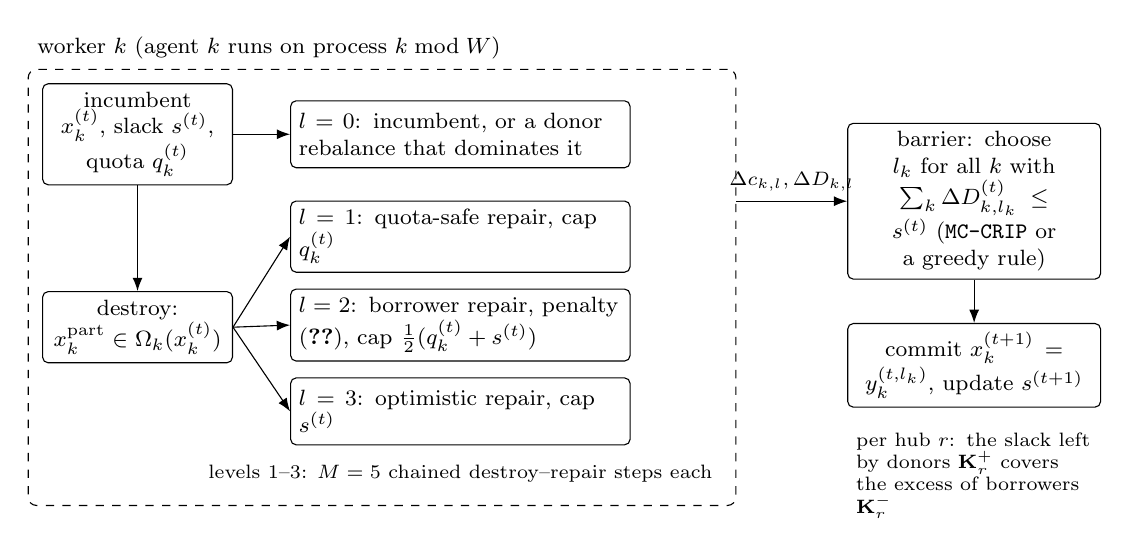
\begin{tikzpicture}[font=\footnotesize, >=Latex,
    box/.style={draw, rounded corners=2pt, align=center, inner sep=3pt},
    lvl/.style={draw, rounded corners=2pt, align=left, inner sep=3pt, text width=4.1cm, minimum height=0.85cm}]
% levels (middle column)
\node[lvl] (l0) at (0, 1.5) {$l=0$: incumbent, or a donor rebalance that dominates it};
\node[lvl] (l1) at (0, 0.2) {$l=1$: quota-safe repair, cap $q_k^{(t)}$};
\node[lvl, below=0.2cm of l1] (l2) {$l=2$: borrower repair, penalty \eqref{eq:surrogate}, cap $\tfrac12(q_k^{(t)}+s^{(t)})$};
\node[lvl, below=0.2cm of l2] (l3) {$l=3$: optimistic repair, cap $s^{(t)}$};
% inputs (left column)
\node[box, text width=2.2cm] (inc) at (-4.1, 1.5) {incumbent $x_k^{(t)}$, slack $s^{(t)}$, quota $q_k^{(t)}$};
\node[box, text width=2.2cm] (part) at (-4.1, -0.95) {destroy: $x_k^{\text{part}} \in \Omega_k(x_k^{(t)})$};
\draw[->] (inc) -- (l0);
\draw[->] (inc) -- (part);
\draw[->] (part.east) -- (l1.west);
\draw[->] (part.east) -- (l2.west);
\draw[->] (part.east) -- (l3.west);
\node[font=\scriptsize, below=0.12cm of l3] (mnote) {levels $1$--$3$: $M = 5$ chained destroy--repair steps each};
\node[draw, dashed, rounded corners=3pt, inner sep=5pt, fit=(inc)(part)(l0)(l3)(mnote)] (worker) {};
\node[font=\footnotesize, anchor=south west] at (worker.north west) {worker $k$ (agent $k$ runs on process $k \bmod W$)};
% barrier (right column)
\node[box, text width=3.0cm, right=2.75cm of l1, yshift=0.45cm] (bar) {barrier: choose $l_k$ for all $k$ with $\sum_k \Delta D_{k,l_k}^{(t)} \le s^{(t)}$ (\mcc{} or a greedy rule)};
\node[box, text width=3.0cm, below=0.55cm of bar] (commit) {commit $x_k^{(t+1)} = y_k^{(t,l_k)}$, update $s^{(t+1)}$};
\draw[->] (worker.east |- bar.west) -- node[above, font=\scriptsize]{$\Delta c_{k,l}, \Delta D_{k,l}$} (bar.west);
\draw[->] (bar) -- (commit);
\node[font=\scriptsize, text width=3.0cm, align=left, below=0.2cm of commit] {per hub $r$: the slack left by donors $\mathbf{K}_r^+$ covers the excess of borrowers $\mathbf{K}_r^-$};
\end{tikzpicture}
\caption{One epoch of \pcm. Level $0$ is derived from the incumbent $x_k^{(t)}$; levels $1$ to $3$ start from the same destroyed solution $x_k^{\text{part}}$ and run $M = 5$ chained destroy--repair steps against their capacity caps. Workers send only scalar cost changes and $m$-dimensional usage changes. The barrier selects one level per worker so that the selection fits into the residual slack; donor and borrower status is defined per hub $r$.}
\label{fig:architecture}
\end{figure}

\subsection{Barrier conflict resolution}
\label{sec:barrier}
At the barrier the coordinator first tries the \emph{fast path}: every worker takes its cheapest level $l_k = \arg\min_l \Delta c_{k,l}^{(t)}$, which is committed if $\sum_k \Delta D_{k,l_k}^{(t)} \le s^{(t)}$. Otherwise the epoch is a \emph{conflict epoch} and a commit rule chooses the selection. Because $\sum_k q_k^{(t)} = s^{(t)}$, the quotas cancel in the barrier constraint: for every hub $r$ and selection $(l_1,\dots,l_K)$,
\begin{equation}
    \sum_{k=1}^{K} \delta_{r,k,l_k}^{(t)} = \sum_{k=1}^{K} D_{r,k}\big(y_k^{(t,l_k)} - x_k^{(t)}\big) - s_r^{(t)}, \label{eq:cancellation}
\end{equation}
so $\sum_k \delta_{r,k,l_k}^{(t)} \le 0$ is equivalent to $\sum_k \Delta D_{r,k,l_k}^{(t)} \le s_r^{(t)}$ whatever the quota shares. Quotas therefore do not restrict the barrier; they act only on the worker side, as trust regions that make levels $1$ and $2$ different from level $3$ and so diversify the portfolio.

\textit{Exact barrier (\mcc).} With $z_{k,l} \in \{0,1\}$,
\begin{equation}
    \min_z \sum_{k=1}^{K}\sum_{l=0}^{L} \Delta c_{k,l}^{(t)} z_{k,l} \quad \text{s.t.} \quad \sum_{k=1}^{K}\sum_{l=0}^{L} \delta_{r,k,l}^{(t)} z_{k,l} \le 0 \ \ (r = 1,\dots,m), \qquad \sum_{l=0}^{L} z_{k,l} = 1 \ \ (k \in \mathbf{K}). \label{eq:mccrip}
\end{equation}
Levels dominated by another level of the same agent are removed. If at most $4{,}096$ level combinations remain, \eqref{eq:mccrip} is solved by enumeration, otherwise by HiGHS \citep{huangfu2018} with relative gap $0$ and a $2$ s limit. If HiGHS reaches the limit without proving optimality, the coordinator commits the cheapest feasible selection among the HiGHS incumbent, the \bcrm{} selection and the all-quota-safe selection $z_{k,1} = 1$. In the experiments this fallback was used in $\FallbackRuns$ of the $100$ XXL and XXXL runs of \pcm{} [\mcc] in Table~\ref{tab:main}, once in each of these runs, and never elsewhere.

\textit{Greedy barriers.} \ggp{} and \gep{} start every worker at level $0$ and scan the upgrades $(k,l)$, $l \ge 1$, with gain $g_{k,l} = \Delta c_{k,0}^{(t)} - \Delta c_{k,l}^{(t)} > 0$ in decreasing order of $g_{k,l}$ or of the efficiency $e_{k,l} = g_{k,l} / (\|[\Delta D_{k,l}^{(t)} - \Delta D_{k,0}^{(t)}]_+\|_1 + 10^{-6})$; an upgrade is committed if the worker is still at level $0$ and the extra usage fits into the remaining slack. \bcrm{} (quota-surplus greedy upgrade) starts every worker at its quota-safe level $1$, which leaves the surplus $S = -\sum_k \delta_{k,1}^{(t)} \ge 0$, and scans the upgrades $(k,l)$, $l \ge 2$, with $\Delta c_{k,l}^{(t)} < \Delta c_{k,1}^{(t)}$ in decreasing order of $\phi_{k,l} = (\Delta c_{k,1}^{(t)} - \Delta c_{k,l}^{(t)}) / (\rho_t \|[\beta_{k,l}]_+\|_2^2 + 10^{-6})$ with $\beta_{k,l} = \delta_{k,l}^{(t)} - \delta_{k,1}^{(t)}$; an upgrade is committed if $\beta_{k,l} \le S$, after which $S \leftarrow S - \beta_{k,l}$. All greedy rules take $O(KL\log(KL) + KLm)$ time.

\textit{Baseline rules.} \texttt{Opt-Rollback} commits all cheapest levels if they fit and otherwise one uniformly chosen improving worker. \texttt{Opt-SeqLock} checks the cheapest levels in a random arrival order $\pi$ and commits each while it fits. \texttt{Static-Quota} commits level $1$ for every worker, and \texttt{Demand-Quota} does the same with shares $\alpha_{r,k}$ proportional to agent $k$'s usage of hub $r$ under its unconstrained cheapest patterns. The single-proposal versions of \texttt{Opt-Rollback} and \texttt{Opt-SeqLock} receive only the optimistic proposal (identical to level $3$); the \texttt{-Portfolio} versions receive the full portfolio and apply the rule to the cheapest level. Algorithm~\ref{alg:epoch} summarizes one epoch.

\begin{algorithm}[!htb]
\caption{Epoch $t$ of \pcm}
\label{alg:epoch}
\small
\begin{algorithmic}[1]
\Require feasible incumbent $x^{(t)}$, slack $s^{(t)}$, penalty $\rho_t$
\State send $(s^{(t)}, q_k^{(t)} = s^{(t)}/K)$ to the $W$ worker processes (agent $k$ runs on process $k \bmod W$)
\ForAll{$k \in \mathbf{K}$ \textbf{in parallel}}
    \State $y_k^{(t,0)} \gets$ donor rebalance of $x_k^{(t)}$ if it dominates $x_k^{(t)}$, else $x_k^{(t)}$
    \State $x_k^{\text{part}} \gets$ destroy $16\%$--$30\%$ of the requests of $x_k^{(t)}$
    \For{$l = 1, 2, 3$} \Comment{caps $q_k^{(t)}$, $\frac12(q_k^{(t)} + s^{(t)})$, $s^{(t)}$}
        \State $y_k^{(t,l)} \gets$ $M$ chained Regret-2 destroy--repair steps from $x_k^{\text{part}}$ (level $2$ minimizes \eqref{eq:surrogate})
        \State \textbf{if} $c_k^\top y_k^{(t,l)} \ge c_k^\top x_k^{(t)}$ \textbf{then} $y_k^{(t,l)} \gets x_k^{(t)}$
    \EndFor
    \State send $(\Delta c_{k,l}^{(t)}, \Delta D_{k,l}^{(t)})_{l=0}^{3}$
\EndFor
\State $l_k \gets \arg\min_l \Delta c_{k,l}^{(t)}$ for all $k$
\If{$\sum_k \Delta D_{k,l_k}^{(t)} \not\le s^{(t)}$} \Comment{conflict epoch}
    \State $(l_1,\dots,l_K) \gets$ optimal solution of \eqref{eq:mccrip} (\mcc) or the selection of a greedy rule
    \State \textbf{if} \mcc{} stopped at its time limit without proof \textbf{then} take the cheapest of its incumbent, \bcrm{} and $l_k = 1\ \forall k$
\EndIf
\State commit $x_k^{(t+1)} \gets y_k^{(t,l_k)}$ for all $k$; \ $s^{(t+1)} \gets d - \sum_k D_k x_k^{(t+1)}$
\end{algorithmic}
\end{algorithm}

\subsection{Properties}
\label{sec:theory}

\begin{proposition}[Global feasibility, monotone descent and per-epoch commit dominance]
\label{prop:main}
Let $x^{(t)}$ be feasible and let every portfolio contain a level $0$ with $\Delta c_{k,0}^{(t)} \le 0$ and $\Delta D_{k,0}^{(t)} \le 0$ and a level $1$ with $y_k^{(t,1)} \in \mathbf{X}_k$, $\Delta c_{k,1}^{(t)} \le 0$ and $\Delta D_{k,1}^{(t)} \le q_k^{(t)}$, where $\sum_k q_k^{(t)} = s^{(t)}$. Then:
\begin{enumerate}[label=(\roman*), noitemsep]
    \item the selection $z_{k,1} = 1$ for all $k$ is feasible for \eqref{eq:mccrip};
    \item every selection that is feasible for \eqref{eq:mccrip}, in particular the selection of every rule of Section~\ref{sec:barrier}, gives a feasible $x^{(t+1)}$;
    \item $C(x^{(t+1)}) \le C(x^{(t)})$ for every rule, and $C(x^{(t+1)}) \le C(x^{(t)}) + \sum_k \Delta c_{k,1}^{(t)}$ for \mcc{} and \bcrm;
    \item for any common portfolio, the cost change of an optimal \mcc{} selection is at most that of \texttt{Static-Quota}, \texttt{Opt-Rollback}, \texttt{Opt-SeqLock} for every arrival order $\pi$, \ggp, \gep{} and \bcrm.
\end{enumerate}
\end{proposition}
\begin{proof}
(i) By \eqref{eq:cancellation}, $\sum_k \delta_{r,k,1}^{(t)} = \sum_k \Delta D_{r,k,1}^{(t)} - s_r^{(t)} \le \sum_k q_{r,k}^{(t)} - s_r^{(t)} = 0$. (ii) By \eqref{eq:cancellation}, feasibility for \eqref{eq:mccrip} means $\sum_k D_{r,k} y_k^{(t,l_k)} \le \sum_k D_{r,k} x_k^{(t)} + s_r^{(t)} = d_r$, and every level lies in $\mathbf{X}_k$. Each rule selects a feasible combination: the fast path and \texttt{Opt-Rollback} commit a batch only if it fits, a single improving move fits because its cap is $s^{(t)}$, \texttt{Opt-SeqLock} and the greedy rules check the remaining slack before every commit, \texttt{Static-Quota} is selection (i), and \bcrm{} starts from (i) and spends only the surplus $S$. (iii) Every level has $\Delta c_{k,l}^{(t)} \le 0$. \mcc{} is optimal and (i) is feasible, so its cost change is at most $\sum_k \Delta c_{k,1}^{(t)}$; \bcrm{} starts from (i) and accepts only upgrades that lower the cost; the time-limit fallback includes (i). (iv) All rules select a feasible solution of \eqref{eq:mccrip} for the same data, and \mcc{} minimizes over all of them.
\end{proof}

Statement (iv) is a per-epoch statement for a common portfolio. Along a run the methods visit different incumbents, so it does not imply that \mcc{} gives the better final solution; Section~\ref{sec:commit} shows that it does not. In our implementation level $3$ is bit-for-bit the optimistic proposal of the single-proposal baselines and level $1$ the \texttt{Static-Quota} proposal, for the same incumbent, seed and epoch (unit tests). The next result bounds how much a rule can lose against \mcc{} in one epoch. For a rule $R$ and a portfolio, let $G_R$ be the cost reduction of its selection and $G^*$ that of \mcc.

\begin{proposition}[Worst-case single-epoch ratios]
\label{prop:ratios}
For every $\varepsilon > 0$ there are portfolios with
(a) $G^* > 0$ and $G_{\texttt{Static-Quota}} = 0$;
(b) $G^* / \mathbb{E}[G_{\texttt{Opt-Rollback}}] = K - 1$ (expectation over the random single commit);
(c) $G^* / G_{\texttt{Opt-SeqLock}}(\pi) = K/(1+\varepsilon)$ for an arrival order $\pi$;
(d) $G^* / G_{\ggp} = 2/(1+\varepsilon)$ with one hub and $m/(1+\varepsilon)$ with $m$ hubs;
(e) $G^* / G_{\gep} = C/2$ for every $C > 2$, so the ratio of \gep{} is unbounded.
\end{proposition}
\begin{proof}
All portfolios use $q_k = s/K$ and level $0$ equal to the incumbent. (a) Two agents, one hub with $s = 1$: agent $1$ has a move with gain $10$ and usage $1$ only at levels $2$ and $3$, agent $2$ has no move; level $1$ of agent $1$ (cap $1/2$) is the incumbent, so \texttt{Static-Quota} gains $0$ while \mcc{} gains $10$. (b) $K$ agents with the same move of gain $1$ and usage $1$, $s = K - 1$: the batch does not fit, \texttt{Opt-Rollback} commits one move, \mcc{} commits $K-1$. (c) $s = K$; every agent has a level with gain $1$ and usage $1$, and the first agent in $\pi$ has a cheapest level with gain $1+\varepsilon$ that uses all of $s$: \texttt{Opt-SeqLock} commits that level and nothing else fits, while \mcc{} commits the $K$ unit moves. (d) One hub with $s = 2$: a move of gain $1+\varepsilon$ and usage $2$ is scanned before two moves of gain $1$ and usage $1$; with $m$ hubs of slack $1$, a move of gain $1+\varepsilon$ that uses all hubs blocks $m$ single-hub moves of gain $1$. (e) One hub with $s = C$: a move of gain $2$ and usage $1$ (efficiency $2$) is scanned before a move of gain $C$ and usage $C$ (efficiency $1$), which then no longer fits. Each construction is verified in \texttt{tests/test\_worst\_case\_bounds.py}.
\end{proof}

Proposition~\ref{prop:ratios} gives lower bounds on the worst-case ratios; we do not claim that they are tight. Case (e) is the classical failure of ratio-greedy knapsack heuristics. The bounds concern single epochs; Section~\ref{sec:commit} measures how often and by how much the rules differ on real portfolios.

\subsection{Optional prices and quotas (ablation only)}
\label{sec:prices}
For the ablation of Section~\ref{sec:ablation} we keep the price and quota components of the previous version of the method. With \emph{heuristic prices}, $\lambda^{(0)}$ are the LP hub duals and $\lambda^{(t+1)} = [(1-\kappa)\lambda^{(t)} + \gamma_t h^{(t)}]_+$ with $h^{(t)} = \sum_k \Delta D_{k,3}^{(t)} - s^{(t)}$, $\kappa = 0.15$ and $\gamma_t = 0.25 \sum_k |\Delta c_{k,3}^{(t)}| / (\|h^{(t)}\|_2^2 + 1)$. With \emph{\mcc{} LP duals}, $\lambda^{(t+1)} = (1-\kappa')\lambda^{(t)} + \kappa' \mu^{(t)}$, $\kappa' = 0.3$, where $\mu^{(t)}$ are the coupling-row duals of the LP relaxation of \eqref{eq:mccrip} in conflict epochs ($\mu^{(t)} = 0$ otherwise). Prices enter the borrower surrogate \eqref{eq:surrogate}, the donor rebalance and the \bcrm{} score. \emph{Dynamic quotas} move the shares towards agents whose optimistic move was blocked: with the unrealized gain $g_k = \max\{0, \Delta c_{k,1}^{(t)} - \Delta c_{k,3}^{(t)}\}$ ($g_k = 0$ if level $3$ was committed) and the excess $e_{r,k} = [\delta_{r,k,3}^{(t)}]_+$,
\begin{equation}
    u_{r,k} = \begin{cases} g_k / e_{r,k} + 10^{-3}, & e_{r,k} > 0, \\ 10^{-3}, & e_{r,k} = 0, \end{cases} \qquad \alpha_{r,k}^{(t+1)} = (1-\omega)\alpha_{r,k}^{(t)} + \omega \frac{u_{r,k}}{\sum_{j=1}^K u_{r,j}}, \quad \omega = 0.25. \label{eq:quota_update}
\end{equation}

\section{Experimental design}
\label{sec:design}

\paragraph{Protocol.} All configuration choices were made on validation instances (seeds $1$ to $10$) that are disjoint from the test instances (seeds $101$ to $110$). A pilot on seeds $1$ to $3$ compared the starts (\texttt{LP-Round}, a decentralized booking start and the direct start with all requests on $p = 0$), the consolidation cap of earlier versions and $M \in \{1,5\}$; \texttt{LP-Round}, no cap and $M = 5$ were best, and on these seeds \mcc{} and \gep{} tied (mean gaps $2.038\%$ and $2.031\%$, exact Wilcoxon $p = 0.84$). \mcc{} was therefore fixed as the primary barrier mode before any test run. The parameters were then tuned on seeds $1$ to $10$ (Section~\ref{sec:ablation}); no change was adopted.

\paragraph{Instances.} RPA-SH instances come from a seeded generator, since no public benchmark exists for this model. The scales are Small, Medium, Large, X-Large, XXL and XXXL with $K = 4, 8, 12, 16, 24, 32$ agents and $N_{\text{agent}} = 30, 40, 50, 60, 100, 125$, i.e.\ $120$ to $4{,}000$ requests. Pattern $0$ costs $c_{k,i,0} \sim U(85,140)$ and uses no capacity. Patterns $p \ge 1$ cost $\theta_{k,i,p} c_{k,i,0}$, where a seeded half of the depots has $\theta \sim U(0.28, 0.52)$ and the other half $\theta \sim U(0.62, 0.85)$; each uses two of $m = 8$ hubs, drawn from the depot's hub profile $\psi_k \sim \text{Dirichlet}(1.5 \cdot \mathbf{1}_m)$, with usage $u (1 + 0.8(1-\theta))$, $u \sim U(1, 3.5)$, and one of $m_{\text{local}} = 4$ waves with usage $U(1, 2.5)$. With $U_r$ the hub-$r$ usage of the unconstrained cheapest patterns, $d_r = \max\{8, U_r/\eta\}$ for the coupling tightness $\eta$, and $b_{k,w} = \max\{4, 0.82 \sum_i A_{w,k,i,p^*_{k,i}}\}$. The main benchmark uses $P = 6$ and $\eta = 1.25$; the rich-pool benchmark (Section~\ref{sec:rich}) uses $P \in \{20, 40\}$ on Medium to XXL.

\textit{RPA-SH-Sync} adds inter-depot transfers. Agents are paired, $(k, k')$ with $k' = k \oplus 1$, and every pair shares a transfer dock with an integer number of slots. For $30\%$ of the requests the last pattern is replaced by a transfer pattern with cost $c_{k,i,0} \cdot U(0.18, 0.32)$ that uses an outbound wave at a hub of agent $k$, an inbound wave at a different hub of agent $k'$ (usage $1.8 \cdot U(1, 3.5)$ each) and a block of $1$, $2$ or $3$ dock slots (probabilities $0.5$, $0.3$, $0.2$). Every dock has $\max\{1, \lfloor U_T/2 \rfloor\}$ slots, $U_T$ being the slot demand of the cheapest patterns. The design was fixed before any run on these instances.

\textit{MMKP benchmarks.} The $27$ classical instances I07--I13 \citep{khan2002} and INST01--INST20 \citep{hifi2006} in the distribution of \citet{chen2014} have $50$ to $400$ groups of $10$ to $30$ items and $10$ resources. Each group becomes a request, the groups are split over $K = 8$ agents in contiguous blocks, item $j$ becomes pattern $j+1$ with cost $\max$ profit $-$ profit, and pattern $0$ has a cost larger than any profit difference, so that a solution with an unassigned group is worse than every MMKP solution. \texttt{LP-Round} leaves at least one group unassigned on $24$ of the $27$ instances, and no LNS method repairs this, because no worker accepts a cost-increasing move. All LNS methods therefore start from the better of \texttt{LP-Round} and the classical two-phase construction of \citet{khan2002} (lightest item per group, then the best feasible upgrades by profit per added normalized weight); its time is charged. On INST04 neither start is feasible. Gaps are measured against the best known values of verified solution certificates.

\paragraph{Methods and budgets.} Table~\ref{tab:methods} lists the methods. All LNS methods share the worker code, the operators ($M = 5$, destroy $16\%$ to $30\%$, Regret-2 with noise $\sigma = 2.0$ and $2.7$ in a best-of-two repair), the random stream of worker $k$ in epoch $t$ and run $\iota \in \{0,\dots,4\}$, and the \texttt{LP-Round} start. They run on a persistent pool of $W = 4$ worker processes; process $w$ owns the agents $k$ with $k \bmod W = w$, keeps their incumbents and portfolios, and exchanges only the per-level cost and usage changes with the coordinator, so the trajectories are identical to serial execution. The wall-clock budgets are $0.5$, $1$, $1.5$, $2$, $4$ and $6$ s from Small to XXXL and include the \texttt{LP-Round} time and shipping the instance to the processes; the one-time process start-up (below $0.5$ s) is not charged. HiGHS 1.8.0 runs in a separate process with relative gap $10^{-4}$. The reference run uses one thread and $600$ s (Small, Medium) or $60$ s (Large to XXXL) in the main benchmark, $30$ s in the rich-pool benchmark and the tightness sweep, and $60$ s on RPA-SH-Sync; HiGHS (5s), HiGHS (60s) and HiGHS (CPU-matched) are read from the incumbent trace of this run. HiGHS (wall-matched) runs separately with one and with four threads and a time limit equal to the mean wall-clock time of the five \pcm{} [\mcc] runs of the instance; HiGHS (CPU-matched) uses their mean CPU time. HiGHS times cover the solver call; building and passing the model took at most $0.04$ s.

\begin{table}[!htb]
\centering
\caption{Compared methods. All LNS methods share workers, operators, random streams and start; they differ in the portfolio and the commit rule.}
\label{tab:methods}
\footnotesize
\begin{tabular}{@{}lll@{}}
\toprule
\textbf{Method} & \textbf{Candidates per worker} & \textbf{Commit rule} \\
\midrule
\pcm{} [\mcc] (primary) & levels $0$--$3$ & exact \eqref{eq:mccrip} \\
\pcm{} [\bcrm] & levels $0$--$3$ & quota-surplus greedy upgrade \\
\gep{} & levels $0$--$3$ & greedy by gain per unit of extra usage \\
\ggp{} & levels $0$--$3$ & greedy by gain \\
\texttt{Opt-Rollback-Portfolio} & levels $0$--$3$ & cheapest level, batch rollback \\
\texttt{Opt-SeqLock-Portfolio} & levels $0$--$3$ & cheapest level, sequential lock \\
\texttt{Opt-Rollback} & optimistic proposal (level $3$) & batch rollback \\
\texttt{Opt-SeqLock} & optimistic proposal (level $3$) & sequential lock \\
\texttt{Static-Quota} & quota-safe proposal, $q_k = s^{(t)}/K$ & commit all \\
\texttt{Demand-Quota} & quota-safe proposal, demand shares & commit all \\
\texttt{LP-Round} & -- & deterministic warm start \\
HiGHS & -- & exact solver, $1$ or $4$ threads \\
\bottomrule
\end{tabular}
\end{table}

\paragraph{Measurements.} The gap is $100 (C(x) - LB)/LB$ with $LB = \max\{$LP bound, dual bound of the reference HiGHS run$\}$; no reference run proved optimality, not even at $600$ s on Small, so the gaps are upper bounds on the true gaps. The primal integral \citep{berthold2013} over the run's wall-clock time uses the primal gap $|C - LB|/\max\{|C|, |LB|\}$, set to $1$ before the first solution. \pcm{} has no solution until the \texttt{LP-Round} start exists and has been shipped to the processes, which takes on average $0.01$ to $0.23$ s with $P = 6$, up to $0.36$ s with $P = 20$ and up to $0.67$ s with $P = 40$ (XXL). We record wall-clock time, CPU time (start plus the sum of worker and barrier times), conflict epochs, and the acceptance rate (committed improving moves per worker with an improving candidate).

\paragraph{Statistics.} The unit of analysis is the instance: the mean of the five runs of an LNS method, and the single value of a deterministic method. For every comparison we report the paired mean difference with Student-$t$ and bootstrap ($10{,}000$ resamples) $95\%$ confidence intervals, wins, ties and losses, and the exact two-sided Wilcoxon signed-rank test (zero differences dropped, mid-ranks, exact conditional null distribution, never a normal approximation), Holm-adjusted within each table. Experiments ran one job at a time on an Apple M4 (4 performance and 6 efficiency cores, 16 GB) with Python 3.11, NumPy 2.3.5, SciPy 1.16.3 and highspy 1.8.0.

\section{Results}
\label{sec:results}

\subsection{Main benchmark}
\label{sec:main}
Table~\ref{tab:main} reports the mean gaps per scale and Table~\ref{tab:main_tests} the pooled comparison with \pcm{} [\mcc]. Starting from \texttt{LP-Round} ($\AGapAllLPRound\%$ over all $60$ instances), \pcm{} [\mcc] reaches $\AGapAllPCMALNSMCCRIP\%$. It beats \texttt{Opt-Rollback} and \texttt{Opt-SeqLock} on $58$ and $56$ of the $60$ instances (mean differences $\ATestOptRollbackDiff$ and $\ATestOptSeqLockDiff$ percentage points, pp) and their portfolio versions on $57$ instances each ($\ATestOptRollbackPortfolioDiff$ and $\ATestOptSeqLockPortfolioDiff$ pp), all with $p_{\text{Holm}} < 10^{-4}$. Giving the optimistic rules the four-level portfolio therefore does not close the gap: the loss comes from the commit rule, not from the candidates. \texttt{Static-Quota} and \texttt{Demand-Quota} lose on all $60$ instances ($\ATestStaticQuotaDiff$ and $\ATestDemandQuotaDiff$ pp). Among the portfolio barriers, \pcm{} [\mcc] is slightly better than \bcrm{} ($\ATestPCMALNSBCRMGreedyWTL$, $\ATestPCMALNSBCRMGreedyDiff$ pp, $p_{\text{Holm}} = \ATestPCMALNSBCRMGreedyP$) and \ggp{} ($\ATestGGPWTL$), but \gep{} is better than \pcm{} [\mcc] on $44$ of $60$ instances ($+\ATestGEPDiff$ pp, $95\%$ CI $\ATestGEPCI$, $p_{\text{Holm}} < 10^{-4}$); Section~\ref{sec:commit} analyses this result.

\begin{table}[!htb]
\centering
\caption{Main benchmark ($P = 6$, $\eta = 1.25$, 10 test instances per scale): mean gap to the lower bound (\%) per scale and mean primal integral (PI, s $\times$ gap fraction) over all 60 instances. LNS methods: mean over 5 runs per instance on $W = 4$ processes with wall-clock budgets of 0.5, 1, 1.5, 2, 4 and 6 s. HiGHS (5s), (60s) and (CPU-matched) are read from the incumbent trace of the 1-thread reference run (600 s on Small and Medium, 60 s otherwise); the wall-matched runs are separate runs with the mean wall-clock time of PC-MALNS [MC-CRIP].}
\label{tab:main}
\footnotesize
\begin{tabular}{@{}lrrrrrrrr@{}}
\toprule
Method & Small & Medium & Large & X-Large & XXL & XXXL & All & PI \\
\midrule
LP-Round & 5.11 & 3.67 & 3.05 & 2.61 & 1.62 & 1.31 & 2.90 & -- \\
\textbf{PC-MALNS [MC-CRIP]} & 2.55 & 1.83 & 1.66 & 1.41 & 0.90 & 0.73 & 1.51 & 0.108 \\
\addlinespace
PC-MALNS [BCRM-Greedy] & 2.57 & 1.87 & 1.65 & 1.42 & 0.91 & 0.74 & 1.53 & 0.106 \\
Greedy-Efficiency-Portfolio & 2.57 & 1.80 & 1.58 & 1.38 & 0.88 & 0.72 & 1.49 & 0.105 \\
Greedy-Gain-Portfolio & 2.62 & 1.83 & 1.66 & 1.45 & 0.95 & 0.80 & 1.55 & 0.107 \\
\addlinespace
Opt-Rollback-Portfolio & 2.75 & 2.04 & 1.82 & 1.57 & 1.05 & 0.88 & 1.69 & 0.112 \\
Opt-SeqLock-Portfolio & 2.63 & 2.03 & 1.81 & 1.57 & 1.00 & 0.82 & 1.64 & 0.109 \\
Opt-Rollback & 2.74 & 2.04 & 1.80 & 1.58 & 1.05 & 0.88 & 1.68 & 0.110 \\
Opt-SeqLock & 2.62 & 2.05 & 1.81 & 1.60 & 1.02 & 0.84 & 1.66 & 0.108 \\
\addlinespace
Static-Quota & 4.18 & 3.11 & 2.61 & 2.23 & 1.39 & 1.14 & 2.44 & 0.120 \\
Demand-Quota & 3.82 & 2.87 & 2.41 & 2.04 & 1.29 & 1.04 & 2.24 & 0.117 \\
\addlinespace
HiGHS (1T, wall-matched) & 1.31 & 1.56 & 3.40 & 3.05 & 1.74 & 1.46 & 2.08 & 0.054 \\
HiGHS (4T, wall-matched) & 1.31 & 1.42 & 3.03 & 2.78 & 1.74 & 1.46 & 1.96 & 0.054 \\
HiGHS (1T, CPU-matched) & 1.11 & 0.69 & 0.47 & 0.40 & 0.23 & 0.18 & 0.51 & 0.109 \\
HiGHS (5s) & 0.90 & 0.69 & 0.47 & 0.45 & 1.74 & 1.46 & 0.95 & 0.081 \\
HiGHS (60s) & 0.59 & 0.42 & 0.36 & 0.34 & 0.22 & 0.16 & 0.35 & 0.318 \\
HiGHS (600s) & 0.47 & 0.32 & -- & -- & -- & -- & 0.40 & 2.686 \\
\bottomrule
\end{tabular}
\end{table}

\begin{table}[!htb]
\centering
\caption{Main benchmark, pooled over the 60 test instances: PC-MALNS [MC-CRIP] (mean gap 1.514\%) against every method. Diff $=$ PC-MALNS [MC-CRIP] $-$ method in percentage points (negative favours PC-MALNS [MC-CRIP]) with paired-$t$ and bootstrap 95\% confidence intervals; W/T/L counts the instances on which PC-MALNS [MC-CRIP] is better, equal or worse; $p$: exact two-sided Wilcoxon signed-rank test, Holm-adjusted over the 16 comparisons.}
\label{tab:main_tests}
\footnotesize
\begin{tabular}{@{}lrrrrrr@{}}
\toprule
Method & Gap & Diff & $t$ 95\% CI & Bootstrap 95\% CI & W/T/L & $p_{\text{Holm}}$ \\
\midrule
LP-Round & 2.896 & $-$1.382 & [$-$1.578, $-$1.187] & [$-$1.574, $-$1.200] & 60/0/0 & $<$0.0001 \\
PC-MALNS [BCRM-Greedy] & 1.526 & $-$0.012 & [$-$0.026, +0.001] & [$-$0.025, +0.001] & 40/0/20 & 0.0336 \\
Greedy-Efficiency-Portfolio & 1.487 & +0.026 & [+0.010, +0.043] & [+0.009, +0.041] & 16/0/44 & $<$0.0001 \\
Greedy-Gain-Portfolio & 1.550 & $-$0.036 & [$-$0.057, $-$0.015] & [$-$0.057, $-$0.016] & 46/0/14 & 0.0012 \\
Opt-Rollback-Portfolio & 1.686 & $-$0.172 & [$-$0.200, $-$0.144] & [$-$0.201, $-$0.145] & 57/0/3 & $<$0.0001 \\
Opt-SeqLock-Portfolio & 1.645 & $-$0.131 & [$-$0.156, $-$0.107] & [$-$0.154, $-$0.107] & 57/0/3 & $<$0.0001 \\
Opt-Rollback & 1.683 & $-$0.169 & [$-$0.200, $-$0.139] & [$-$0.199, $-$0.140] & 58/0/2 & $<$0.0001 \\
Opt-SeqLock & 1.659 & $-$0.145 & [$-$0.172, $-$0.118] & [$-$0.172, $-$0.119] & 56/0/4 & $<$0.0001 \\
Static-Quota & 2.443 & $-$0.929 & [$-$1.050, $-$0.808] & [$-$1.046, $-$0.814] & 60/0/0 & $<$0.0001 \\
Demand-Quota & 2.244 & $-$0.730 & [$-$0.826, $-$0.634] & [$-$0.823, $-$0.639] & 60/0/0 & $<$0.0001 \\
HiGHS (1T, wall-matched) & 2.084 & $-$0.570 & [$-$0.887, $-$0.254] & [$-$0.871, $-$0.261] & 44/0/16 & 0.0089 \\
HiGHS (4T, wall-matched) & 1.956 & $-$0.443 & [$-$0.760, $-$0.125] & [$-$0.746, $-$0.133] & 41/0/19 & 0.0336 \\
HiGHS (1T, CPU-matched) & 0.512 & +1.001 & [+0.907, +1.096] & [+0.912, +1.096] & 0/0/60 & $<$0.0001 \\
HiGHS (5s) & 0.951 & +0.562 & [+0.304, +0.820] & [+0.309, +0.810] & 20/0/40 & $<$0.0001 \\
HiGHS (60s) & 0.348 & +1.166 & [+1.036, +1.295] & [+1.043, +1.293] & 0/0/60 & $<$0.0001 \\
HiGHS (600s) & 0.398 & +1.792 & [+1.617, +1.966] & [+1.638, +1.954] & 0/0/20 & $<$0.0001 \\
\bottomrule
\end{tabular}
\end{table}


Against HiGHS the picture depends on the budget (Figure~\ref{fig:gap_scale}). With the same wall-clock time, \pcm{} [\mcc] is better than HiGHS with one thread on $44$ of $60$ instances ($\ATestHiGHSOneTwallmatchedDiff$ pp, $p_{\text{Holm}} = \ATestHiGHSOneTwallmatchedP$) and with four threads on $41$ ($\ATestHiGHSFourTwallmatchedDiff$ pp, $p_{\text{Holm}} = \ATestHiGHSFourTwallmatchedP$). The advantage is confined to Large and above: on Small and Medium, HiGHS is better already at $0.5$ to $1$ s. HiGHS with $5$ s is better on Small to X-Large, but on XXL and XXXL its incumbent at $5$ s ($1.74\%$ and $1.46\%$) is still worse than that of \pcm; HiGHS with $60$ s and HiGHS with the same CPU time are better on all $60$ instances. HiGHS with four threads hardly differs from one thread, as its branch and bound is essentially sequential. The primal integral of wall-matched HiGHS is lower than that of \pcm{} on the larger scales despite its worse final gap, because HiGHS finds a first, weak incumbent almost immediately while \pcm{} has no solution before its start exists (Figure~\ref{fig:anytime}).

\begin{figure}[!htb]
\centering
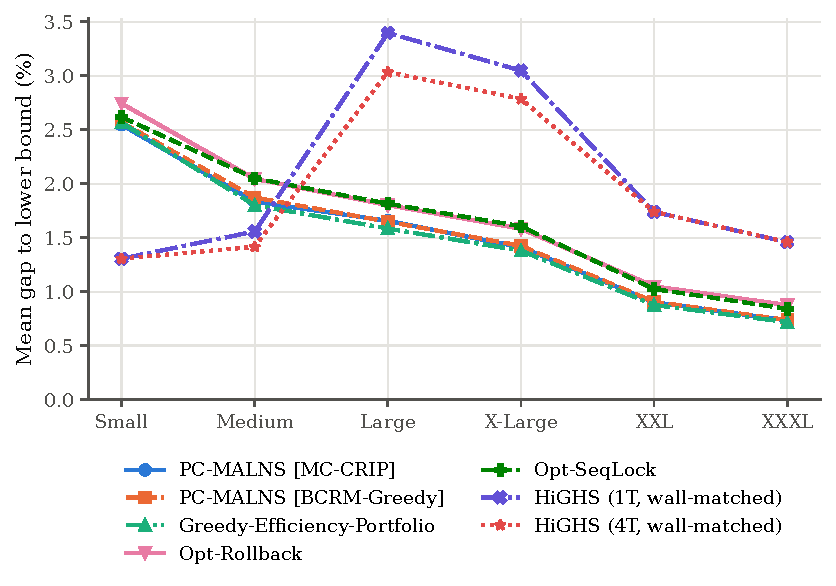
\includegraphics{../results/figures/fig_gap_by_scale.pdf}
\caption{Mean gap to the lower bound by scale ($P = 6$, $\eta = 1.25$; LNS methods: mean over $5$ runs per instance on $W = 4$ processes; HiGHS with the same wall-clock time).}
\label{fig:gap_scale}
\end{figure}

\begin{figure}[!htb]
\centering
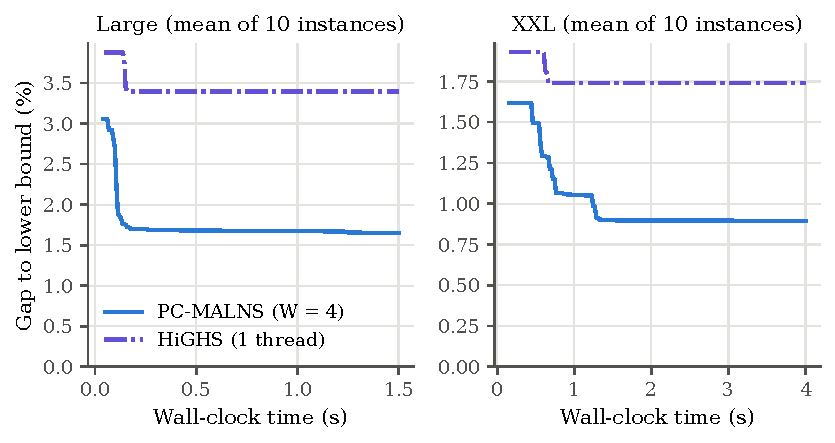
\includegraphics{../results/figures/fig_anytime.pdf}
\caption{Anytime behaviour on Large and XXL ($P = 6$): mean gap of \pcm{} [\mcc] (run $0$, $W = 4$) and of the 1-thread HiGHS reference run over wall-clock time. Each curve starts once every instance has a solution.}
\label{fig:anytime}
\end{figure}

\subsection{Rich candidate pools}
\label{sec:rich}
With $20$ or $40$ candidates per request (Table~\ref{tab:rich}, Figure~\ref{fig:rich}), the integer program grows to $20$ or $40$ binaries per request, and HiGHS with the same wall-clock time does not improve its incumbent within these limits (its CPU-matched incumbent is the same). \pcm{} [\mcc] reaches $\BPTwoZeroGapAllPCMALNSMCCRIP\%$ ($P = 20$) and $\BPFourZeroGapAllPCMALNSMCCRIP\%$ ($P = 40$), against $\BPTwoZeroGapAllHiGHSOneTwallmatched\%$ and $\BPFourZeroGapAllHiGHSOneTwallmatched\%$ for wall-matched HiGHS, and is better on $40$ of $40$ instances for each $P$, with one or four threads and also against HiGHS with the same CPU time ($p_{\text{Holm}} < 10^{-4}$). HiGHS with $30$ s is better at $P = 20$ ($\BPTwoZeroTestHiGHSThreeZerosWTL$, $p_{\text{Holm}} = \BPTwoZeroTestHiGHSThreeZerosP$) and not significantly different at $P = 40$ ($\BPFourZeroGapAllHiGHSThreeZeros\%$ against $\BPFourZeroGapAllPCMALNSMCCRIP\%$, $p_{\text{Holm}} = \BPFourZeroTestHiGHSThreeZerosP$). As on $P = 6$, \gep{} is slightly better than \pcm{} [\mcc] ($+\BPTwoZeroTestGEPDiff$ and $+\BPFourZeroTestGEPDiff$ pp) and \pcm{} [\mcc] beats the optimistic rules on $38$ to $40$ of $40$ instances. The primal-integral comparison favours wall-matched HiGHS (Table~\ref{tab:rich}): \pcm{} pays $0.04$ to $0.67$ s of start-up during which its primal gap is $1$ by definition, which outweighs its better final gap within budgets of $1$ to $4$ s. We therefore claim an advantage in final gap, not in primal integral.

\begin{table}[!htb]
\centering
\caption{Rich candidate pools ($P \in \{20, 40\}$, 10 test instances per scale and $P$): mean gap (\%) per scale and over all 40 instances (All), mean primal integral (PI), and the pooled comparison of PC-MALNS [MC-CRIP] with each method (Diff in percentage points, W/T/L, exact Wilcoxon $p$ Holm-adjusted within each $P$). Wall-clock budgets as in Table~\ref{tab:main}; HiGHS (30s) is the 1-thread reference run.}
\label{tab:rich}
\footnotesize
\resizebox{\textwidth}{!}{\begin{tabular}{@{}lrrrrrrrrr@{}}
\toprule
Method & Medium & Large & X-Large & XXL & All & PI & Diff & W/T/L & $p_{\text{Holm}}$ \\
\midrule
\multicolumn{10}{@{}l}{\textit{$P = 20$}} \\
LP-Round & 4.50 & 3.66 & 3.01 & 1.89 & 3.26 & -- & $-$1.001 & 40/0/0 & $<$0.0001 \\
\textbf{PC-MALNS [MC-CRIP]} & 3.00 & 2.51 & 2.14 & 1.40 & 2.26 & 0.195 & & & \\
PC-MALNS [BCRM-Greedy] & 3.03 & 2.52 & 2.15 & 1.37 & 2.27 & 0.195 & $-$0.004 & 21/0/19 & 0.6656 \\
Greedy-Efficiency-Portfolio & 2.91 & 2.49 & 2.09 & 1.36 & 2.21 & 0.194 & +0.051 & 5/0/35 & $<$0.0001 \\
Opt-Rollback & 3.21 & 2.79 & 2.39 & 1.55 & 2.49 & 0.198 & $-$0.223 & 39/0/1 & $<$0.0001 \\
Opt-SeqLock & 3.21 & 2.83 & 2.38 & 1.56 & 2.50 & 0.197 & $-$0.232 & 39/0/1 & $<$0.0001 \\
HiGHS (1T, wall-matched) & 5.38 & 4.27 & 3.44 & 2.16 & 3.81 & 0.063 & $-$1.549 & 40/0/0 & $<$0.0001 \\
HiGHS (4T, wall-matched) & 5.38 & 4.27 & 3.44 & 2.16 & 3.81 & 0.063 & $-$1.549 & 40/0/0 & $<$0.0001 \\
HiGHS (1T, CPU-matched) & 5.38 & 4.27 & 3.44 & 2.16 & 3.81 & 0.229 & $-$1.549 & 40/0/0 & $<$0.0001 \\
HiGHS (30s) & 1.79 & 2.07 & 0.67 & 0.95 & 1.37 & 0.727 & +0.895 & 11/0/29 & 0.0026 \\
\midrule
\multicolumn{10}{@{}l}{\textit{$P = 40$}} \\
LP-Round & 4.62 & 3.51 & 2.90 & 1.77 & 3.20 & -- & $-$0.957 & 40/0/0 & $<$0.0001 \\
\textbf{PC-MALNS [MC-CRIP]} & 3.03 & 2.47 & 2.11 & 1.37 & 2.25 & 0.323 & & & \\
PC-MALNS [BCRM-Greedy] & 3.02 & 2.47 & 2.18 & 1.37 & 2.26 & 0.322 & $-$0.014 & 26/0/14 & 0.1450 \\
Greedy-Efficiency-Portfolio & 2.95 & 2.42 & 2.12 & 1.36 & 2.21 & 0.322 & +0.033 & 14/0/26 & 0.0167 \\
Opt-Rollback & 3.23 & 2.73 & 2.41 & 1.55 & 2.48 & 0.325 & $-$0.234 & 38/0/2 & $<$0.0001 \\
Opt-SeqLock & 3.28 & 2.79 & 2.38 & 1.55 & 2.50 & 0.325 & $-$0.251 & 40/0/0 & $<$0.0001 \\
HiGHS (1T, wall-matched) & 5.72 & 4.44 & 3.85 & 2.41 & 4.11 & 0.062 & $-$1.861 & 40/0/0 & $<$0.0001 \\
HiGHS (4T, wall-matched) & 5.72 & 4.44 & 3.85 & 2.44 & 4.11 & 0.062 & $-$1.869 & 40/0/0 & $<$0.0001 \\
HiGHS (1T, CPU-matched) & 5.72 & 4.44 & 3.85 & 2.41 & 4.11 & 0.236 & $-$1.861 & 40/0/0 & $<$0.0001 \\
HiGHS (30s) & 3.69 & 3.56 & 1.23 & 2.41 & 2.72 & 0.968 & $-$0.477 & 28/0/12 & 0.4680 \\
\bottomrule
\end{tabular}}
\end{table}


\begin{figure}[!htb]
\centering
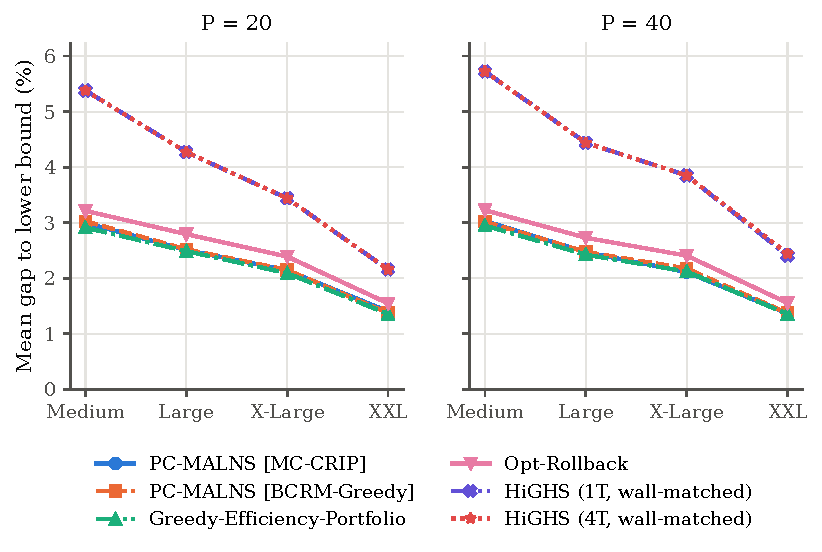
\includegraphics{../results/figures/fig_rich_pools.pdf}
\caption{Mean gap with rich candidate pools ($P = 20$ and $P = 40$). HiGHS runs with the mean wall-clock time of \pcm{} [\mcc]; one and four threads give almost identical results.}
\label{fig:rich}
\end{figure}

\subsection{Commit-rule isolation: exact versus greedy barriers}
\label{sec:commit}
Table~\ref{tab:commit} compares the commit rules on Medium and Large under the \texttt{LP-Round} start, under the direct start with all requests on $p = 0$, which raises the share of conflict epochs to $26.5\%$, and on RPA-SH-Sync. Three results hold in all three regimes. First, \pcm{} [\mcc] beats every optimistic rule, with or without the portfolio, on $19$ or $20$ of $20$ instances (under the direct start by $1.3$ to $2.9$ pp). Second, \pcm{} [\mcc] has the lowest conflict rate of the portfolio rules. Third, \gep{} finishes better than \pcm{} [\mcc]: by $\CLPRoundstartTestGEPDiff$ pp under the \texttt{LP-Round} start ($p_{\text{Holm}} = \CLPRoundstartTestGEPP$), $\CDirectstartTestGEPDiff$ pp under the direct start ($p_{\text{Holm}} = \CDirectstartTestGEPP$) and $\CRPASHSyncTestGEPDiff$ pp on RPA-SH-Sync ($p_{\text{Holm}} = \CRPASHSyncTestGEPP$). Under the direct start \bcrm{} is also better than \mcc, while \mcc{} beats \ggp{} ($\CDirectstartTestGGPWTL$). The transfer-synchronised instances, designed to challenge greedy rules with paired, lumpy dock capacities, do not change the ranking: \mcc{} ties \bcrm{} and \ggp{} and loses to \gep.

\begin{table}[!htb]
\centering
\caption{Commit-rule isolation (Medium and Large, 20 test instances per regime, 5 runs per instance). All rules see the same workers and operators; the portfolio rules see the same four-level portfolio. Gap: mean gap (\%); Conf.: share of epochs in which the cheapest levels do not fit (\%); Diff: PC-MALNS [MC-CRIP] $-$ rule (percentage points; negative favours MC-CRIP); W/T/L of PC-MALNS [MC-CRIP]; $^{*}$: exact Wilcoxon $p < 0.05$ after Holm adjustment within the regime.}
\label{tab:commit}
\footnotesize
\resizebox{\textwidth}{!}{\begin{tabular}{@{}lrrrrrrrrrrrr@{}}
\toprule
 & \multicolumn{4}{c}{LP-Round start} & \multicolumn{4}{c}{Direct start} & \multicolumn{4}{c}{RPA-SH-Sync (LP-Round start)} \\
\cmidrule(lr){2-5}\cmidrule(lr){6-9}\cmidrule(l){10-13}
Rule & Gap & Conf. & Diff & W/T/L & Gap & Conf. & Diff & W/T/L & Gap & Conf. & Diff & W/T/L \\
\midrule
\textbf{PC-MALNS [MC-CRIP]} & 1.74 & 7.7 & &  & 5.98 & 26.5 & &  & 2.12 & 13.4 & &  \\
PC-MALNS [BCRM-Greedy] & 1.76 & 10.6 & $-$0.016 & 15/0/5 & 5.73 & 32.4 & +0.257 & 3/0/17$^{*}$ & 2.12 & 17.7 & $-$0.002 & 9/0/11 \\
Greedy-Efficiency-Portfolio & 1.69 & 10.3 & +0.052 & 7/0/13$^{*}$ & 5.54 & 31.0 & +0.443 & 4/0/16$^{*}$ & 2.03 & 16.8 & +0.084 & 5/0/15$^{*}$ \\
Greedy-Gain-Portfolio & 1.75 & 9.3 & $-$0.001 & 11/0/9 & 6.21 & 30.8 & $-$0.222 & 15/0/5$^{*}$ & 2.13 & 15.5 & $-$0.009 & 12/0/8 \\
Opt-Rollback-Portfolio & 1.93 & 27.9 & $-$0.186 & 20/0/0$^{*}$ & 8.92 & 80.1 & $-$2.934 & 20/0/0$^{*}$ & 2.33 & 46.3 & $-$0.209 & 20/0/0$^{*}$ \\
Opt-SeqLock-Portfolio & 1.92 & 12.9 & $-$0.178 & 20/0/0$^{*}$ & 7.77 & 34.5 & $-$1.786 & 20/0/0$^{*}$ & 2.28 & 19.0 & $-$0.164 & 19/0/1$^{*}$ \\
Opt-Rollback & 1.92 & 11.4 & $-$0.179 & 20/0/0$^{*}$ & 7.27 & 36.5 & $-$1.285 & 19/0/1$^{*}$ & 2.32 & 18.5 & $-$0.198 & 20/0/0$^{*}$ \\
Opt-SeqLock & 1.93 & 5.6 & $-$0.188 & 20/0/0$^{*}$ & 7.56 & 15.8 & $-$1.578 & 20/0/0$^{*}$ & 2.30 & 8.1 & $-$0.183 & 20/0/0$^{*}$ \\
\bottomrule
\end{tabular}}
\end{table}


Table~\ref{tab:counterfactual} explains why this is surprising. On each of the \CFTotalEpochs{} conflict epochs of the \mcc{} runs, every rule was applied to the same portfolios. \mcc{} is strictly better than \gep{} in about half of these epochs and than \ggp{} in $38\%$ to $43\%$; \gep{} obtains only $83\%$ to $84\%$ of the \mcc{} cost reduction, so the exact barrier gains about $20\%$ more per conflict epoch. The optimistic rules obtain $11\%$ to $86\%$ and \texttt{Static-Quota} as little as $6\%$ (Figure~\ref{fig:counterfactual}). The per-epoch dominance of Proposition~\ref{prop:main}(iv) is thus large in practice, yet it does not carry over to the final solutions.

\begin{table}[!htb]
\centering
\caption{Counterfactual barrier analysis. On every conflict epoch of the PC-MALNS [MC-CRIP] runs of Table~\ref{tab:commit} (409, 1,109 and 437 epochs, 1,955 in total), every rule is applied to the same portfolios. Share: total cost reduction of the rule as a percentage of the MC-CRIP reduction; Strict: percentage of these epochs in which MC-CRIP is strictly better. Counterfactual evaluations use their own random stream and are not charged to any clock.}
\label{tab:counterfactual}
\footnotesize
\begin{tabular}{@{}lrrrrrr@{}}
\toprule
 & \multicolumn{2}{c}{LP-Round start} & \multicolumn{2}{c}{Direct start} & \multicolumn{2}{c}{RPA-SH-Sync} \\
\cmidrule(lr){2-3}\cmidrule(lr){4-5}\cmidrule(l){6-7}
Rule & Share & Strict & Share & Strict & Share & Strict \\
\midrule
BCRM-Greedy & 79.6 & 58.2 & 95.5 & 54.3 & 76.9 & 61.3 \\
Greedy-Efficiency & 84.0 & 51.3 & 84.1 & 47.6 & 83.2 & 52.9 \\
Greedy-Gain & 83.9 & 43.0 & 93.1 & 37.8 & 84.3 & 39.4 \\
Opt-SeqLock & 57.4 & 100.0 & 85.9 & 100.0 & 60.4 & 99.8 \\
Opt-Rollback & 20.6 & 100.0 & 10.6 & 100.0 & 19.4 & 100.0 \\
Static-Quota & 6.3 & 100.0 & 74.5 & 100.0 & 5.8 & 100.0 \\
\bottomrule
\end{tabular}
\end{table}


\begin{figure}[!htb]
\centering
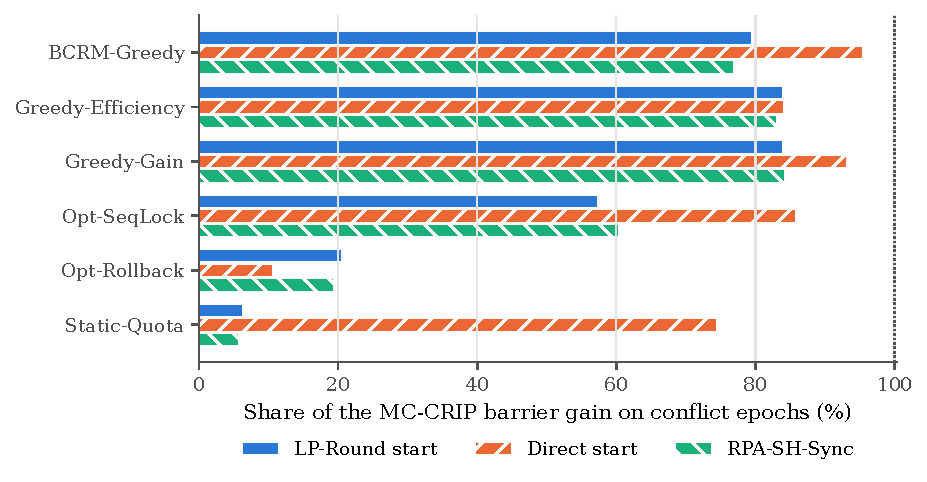
\includegraphics{../results/figures/fig_counterfactual.pdf}
\caption{Share of the \mcc{} cost reduction obtained by each rule on the same portfolios, over all conflict epochs of the \pcm{} [\mcc] runs in Table~\ref{tab:commit}.}
\label{fig:counterfactual}
\end{figure}

\textit{Mechanism.} To see why per-epoch optimality does not pay off, we reran \pcm{} [\mcc], \bcrm{} and \gep{} on the instances of Table~\ref{tab:commit} with the same budgets and logged the residual hub slack after every epoch (Table~\ref{tab:slack}; these are separate runs, and $80\%$ of the \texttt{LP-Round} runs reproduce Table~\ref{tab:main} exactly, the others differ by $0.004$ pp on average because wall-clock budgets shift the last epoch). \mcc{} keeps less slack than \gep{} on $19$ of $20$ instances under both starts (time-averaged mean slack $0.54\%$ against $0.61\%$ of capacity with the warm start, $2.51\%$ against $3.08\%$ with the direct start; exact Wilcoxon $p < 10^{-4}$), less slack on the scarcest hub on $14$ and $16$ of $20$ instances ($p = 0.005$ and $0.004$), and it commits about a quarter fewer improving moves per epoch ($0.33$ against $0.41$ and $1.10$ against $1.36$). This is consistent with the following explanation: in a conflict epoch \mcc{} packs the residual slack into the combination of moves with the largest immediate gain, which often includes capacity-hungry moves, whereas sorting by gain per unit of capacity spends slack on frugal moves first and leaves capacity that later epochs, with new destroyed neighborhoods, turn into further gains. The diagnostic shows an association, not a causal proof; a barrier that values residual slack, for instance by a look-ahead penalty, would be needed to test it directly.

\begin{table}[!htb]
\centering
\caption{Residual hub slack along the trajectory (Medium and Large, 20 test instances, 5 runs each; separate diagnostic runs with the budgets of Table~\ref{tab:commit}). Slack: time average over the epochs of $\frac{1}{m}\sum_r s_r^{(t)}/d_r$ (\%); Bottleneck: time average of $\min_r s_r^{(t)}/d_r$ (\%); Acc./epoch: committed improving worker moves per epoch; Conf.: conflict epochs (\%).}
\label{tab:slack}
\footnotesize
\begin{tabular}{@{}lrrrrrr@{}}
\toprule
Rule & Gap & Slack & Bottleneck & Epochs & Acc./epoch & Conf. \\
\midrule
\multicolumn{7}{@{}l}{\textit{LP-Round start}} \\
\textbf{PC-MALNS [MC-CRIP]} & 1.745 & 0.54 & 0.068 & 58.2 & 0.33 & 7.2 \\
PC-MALNS [BCRM-Greedy] & 1.760 & 0.61 & 0.082 & 59.1 & 0.43 & 9.6 \\
Greedy-Efficiency-Portfolio & 1.693 & 0.61 & 0.080 & 58.8 & 0.41 & 9.3 \\
\multicolumn{7}{@{}l}{\textit{Direct start}} \\
\textbf{PC-MALNS [MC-CRIP]} & 5.923 & 2.51 & 2.062 & 51.7 & 1.10 & 23.8 \\
PC-MALNS [BCRM-Greedy] & 5.688 & 2.67 & 2.034 & 53.3 & 1.34 & 27.9 \\
Greedy-Efficiency-Portfolio & 5.480 & 3.08 & 2.249 & 52.9 & 1.36 & 26.7 \\
\bottomrule
\end{tabular}
\end{table}


We keep \pcm{} [\mcc] as the primary mode in all tables because it was fixed on the validation instances, on which it tied \gep{}; choosing \gep{} after seeing the test results would be a selection on test data. The practical recommendation is nevertheless clear: the cheap efficiency rule is at least as good as the exact barrier at no solver cost, and a new validation study should confirm it as the default.

\subsection{Public MMKP benchmarks: a structural limit}
\label{sec:mmkp}
Table~\ref{tab:mmkp} reports the MMKP results. All LNS methods end between $\DGapAllPCMALNSMCCRIP\%$ and $\DGapAllStaticQuota\%$ from the best known solutions, against $\DGapAllHiGHSOneTwallmatched\%$ for HiGHS with the same wall-clock time and $\DGapAllHiGHSSixZeros\%$ with $60$ s. \pcm{} improves its start on $17$ of the $26$ instances with a feasible start (mean gap from $2.91\%$ to $2.59\%$) and then stalls; conflict epochs occur in fewer than $0.5\%$ of the epochs, so the barrier rules hardly differ, and only \texttt{Static-Quota} is significantly worse. The reason is structural. Every worker filters out candidates that raise its own cost ($\Delta c_{k,l}^{(t)} > 0$), which guarantees monotone descent (Proposition~\ref{prop:main}(iii)); once the start has nearly filled the knapsack capacities, an improvement needs some groups to switch to lighter, more expensive items so that others can upgrade. No worker proposes such a sacrifice, with or without prices, so the search cannot trade capacity between agents. Dedicated MMKP methods \citep{chen2014, gao2017, mansini2020, lamanna2022} reach the best known values; we report these instances as a boundary of the method, not as a competitive benchmark.

\begin{table}[!htb]
\centering
\caption{Public MMKP benchmarks (I07--I13 and INST01--INST20, groups split over $K = 8$ agents; 2 s wall clock on $W = 4$ processes; 5 runs per instance). Gap to the best known solution (\%, MMKP-feasible runs only), share of MMKP-feasible runs (\%), conflict epochs (\%), and the comparison of PC-MALNS [MC-CRIP] with each method (26 instances with a feasible start; Holm-adjusted exact Wilcoxon).}
\label{tab:mmkp}
\footnotesize
\resizebox{\textwidth}{!}{\begin{tabular}{@{}lrrrrrrrr@{}}
\toprule
Method & I07--I13 & INST01--20 & All & Feasible & Conf. & Diff & W/T/L & $p_{\text{Holm}}$ \\
\midrule
\textbf{PC-MALNS [MC-CRIP]} & 2.948 & 2.463 & 2.594 & 96.3 & 0.38 &  &  &  \\
PC-MALNS [BCRM-Greedy] & 2.980 & 2.481 & 2.615 & 96.3 & 0.44 & $-$0.022 & 7/15/4 & 0.5244 \\
Opt-Rollback & 2.919 & 2.513 & 2.622 & 96.3 & 0.29 & $-$0.029 & 8/11/7 & 0.6056 \\
Opt-SeqLock & 2.961 & 2.466 & 2.599 & 96.3 & 0.21 & $-$0.006 & 7/12/7 & 0.7148 \\
Static-Quota & 3.131 & 2.828 & 2.909 & 96.3 & 0.00 & $-$0.316 & 17/9/0 & $<$0.0001 \\
HiGHS (1T, wall-matched) & 0.089 & 0.233 & 0.195 & 100.0 & -- & +2.406 & 0/0/26 & $<$0.0001 \\
HiGHS (4T, wall-matched) & 0.089 & 0.233 & 0.195 & 100.0 & -- & +2.407 & 0/0/26 & $<$0.0001 \\
HiGHS (60s) & 0.049 & 0.152 & 0.125 & 100.0 & -- & +2.475 & 0/0/26 & $<$0.0001 \\
\bottomrule
\end{tabular}}
\end{table}


\subsection{Tightness, ablation, tuning and scaling}
\label{sec:ablation}
\textit{Coupling tightness.} Table~\ref{tab:sweep} and Figure~\ref{fig:tightness} vary $\eta$ on Large. With loose coupling ($\eta = 0.85$), the optimistic single-proposal rules are better than \pcm{} ($1.70\%$ against $1.80\%$, 9 and 8 of 10 instances, unadjusted $p = 0.006$ and $0.014$); the portfolio pays off once the hubs bind ($\eta \ge 1.25$), where \pcm{} beats them on 9 or 10 of 10 instances. At $\eta \ne 1.25$, \gep{} and \pcm{} [\mcc] do not differ significantly. With $40$ tests and $10$ instances per $\eta$, the smallest attainable Holm-adjusted $p$-value is $0.076$, so no comparison of the sweep is significant after adjustment; this family was fixed before the runs.

\begin{table}[!htb]
\centering
\caption{Coupling tightness sweep (Large, 10 test instances per $\eta$; $\eta = 1.25$ from Table~\ref{tab:main}): mean gap (\%).}
\label{tab:sweep}
\footnotesize
\begin{tabular}{@{}lrrrr@{}}
\toprule
Method & $\eta = 0.85$ & $\eta = 1.05$ & $\eta = 1.25$ & $\eta = 1.45$ \\
\midrule
LP-Round & 2.93 & 3.06 & 3.05 & 1.71 \\
\textbf{PC-MALNS [MC-CRIP]} & 1.80 & 1.84 & 1.66 & 1.11 \\
PC-MALNS [BCRM-Greedy] & 1.80 & 1.85 & 1.65 & 1.13 \\
Greedy-Efficiency-Portfolio & 1.79 & 1.85 & 1.58 & 1.10 \\
Opt-Rollback & 1.70 & 1.82 & 1.80 & 1.21 \\
Opt-SeqLock & 1.70 & 1.79 & 1.81 & 1.22 \\
Static-Quota & 1.74 & 2.55 & 2.61 & 1.63 \\
HiGHS (1T, wall-matched) & 0.95 & 3.62 & 3.40 & 0.45 \\
HiGHS (1T, CPU-matched) & 0.32 & 0.47 & 0.47 & 0.41 \\
\bottomrule
\end{tabular}
\end{table}


\begin{figure}[!htb]
\centering
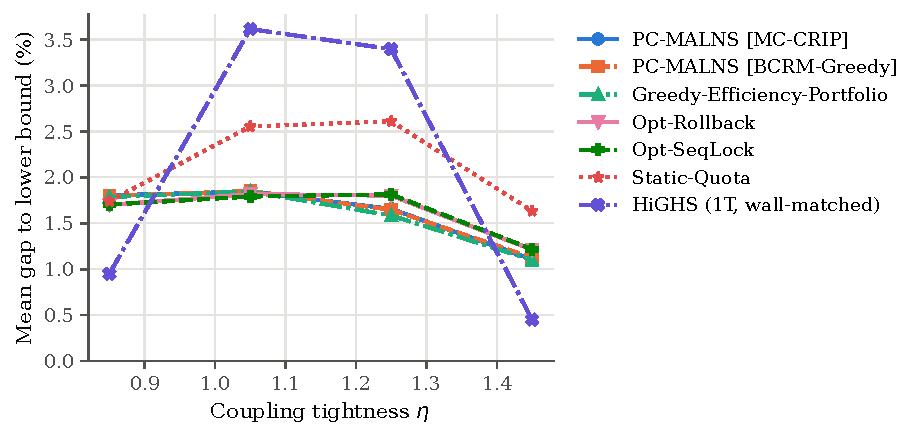
\includegraphics{../results/figures/fig_tightness.pdf}
\caption{Mean gap on Large as a function of the coupling tightness $\eta$.}
\label{fig:tightness}
\end{figure}

\textit{Prices and quotas.} Table~\ref{tab:ablation} adds the price and quota components of Section~\ref{sec:prices} to \pcm{} [\mcc]. None of the six variants differs significantly from the default ($p_{\text{Holm}} = 1.0$ for all); five are nominally better by $0.02$ to $0.03$ pp (on 6 of 10 instances) and the dynamic quota without prices is nominally worse. Because the barrier constraint does not depend on the quotas \eqref{eq:cancellation} and the portfolio already offers the barrier a quota-safe, a borrowing and an optimistic version of every move, steering the borrower repair by prices or reallocating quotas adds no information that the barrier does not already use. We therefore treat prices and dynamic quotas as optional components and omit them from \pcm.

\begin{table}[!htb]
\centering
\caption{Price and quota ablation of PC-MALNS [MC-CRIP] (Large, $\eta = 1.25$, 10 test instances, 5 runs each): mean gap (\%), difference default $-$ variant, W/T/L of the default, exact Wilcoxon $p$ Holm-adjusted over the six variants.}
\label{tab:ablation}
\footnotesize
\begin{tabular}{@{}lrrrr@{}}
\toprule
Variant & Gap & Diff & W/T/L & $p_{\text{Holm}}$ \\
\midrule
No prices, static quota (default) & 1.656 & & & \\
Heuristic prices, dynamic quota & 1.629 & +0.028 & 4/0/6 & 1.0000 \\
Heuristic prices, static quota & 1.632 & +0.024 & 4/0/6 & 1.0000 \\
MC-CRIP LP duals, dynamic quota & 1.627 & +0.029 & 4/0/6 & 1.0000 \\
MC-CRIP LP duals, static quota & 1.635 & +0.021 & 4/0/6 & 1.0000 \\
No prices, demand quota & 1.634 & +0.022 & 4/0/6 & 1.0000 \\
No prices, dynamic quota & 1.662 & $-$0.006 & 7/1/2 & 1.0000 \\
\bottomrule
\end{tabular}
\end{table}


\textit{Parameters.} Table~\ref{tab:tuning} reports the one-factor-at-a-time sensitivity on the validation seeds. No level qualified to replace the default under the pre-declared rule; $M = 10$ came closest ($p_{\text{Holm}} = 0.083$), and a single step ($M = 1$) was worst. Results are insensitive to the destroy range, the noise and $\rho_0$ within the tested ranges.

\begin{table}[!htb]
\centering
\caption{Parameter sensitivity on the validation seeds 1--10 (Medium, 3 runs each, 2 s CPU budget, one factor at a time around the default in bold): level: mean gap (\%) (Holm-adjusted exact Wilcoxon $p$ against the default over 30 paired runs). A level would replace the default only if it were better with $p_{\text{Holm}} < 0.05$; no level qualified.}
\label{tab:tuning}
\footnotesize
\begin{tabular}{@{}lp{0.72\textwidth}@{}}
\toprule
Factor & Levels \\
\midrule
Chained steps $M$ & 1: 1.938 (0.0832); 2: 1.910 (0.1579); \textbf{5: 1.851}; 10: 1.799 (0.0832) \\
Destroy fraction range & [0.08, 0.16]: 1.818 (0.4733); \textbf{[0.16, 0.3]: 1.851}; [0.3, 0.45]: 1.908 (0.4733) \\
Regret-2 noise $\sigma$ & 0.0: 1.846 (1.0000); 1.0: 1.863 (1.0000); \textbf{2.0: 1.851}; 4.0: 1.793 (0.2197) \\
Borrower penalty $\rho_0$ & 0.0: 1.874 (1.0000); 0.15: 1.872 (1.0000); \textbf{0.35: 1.851}; 0.7: 1.813 (1.0000) \\
\bottomrule
\end{tabular}
\end{table}


\textit{Parallel scaling.} Table~\ref{tab:scaling} and Figure~\ref{fig:scaling} report the measured wall clock for a fixed number of epochs. Four processes give a speedup of $2.18$ to $2.37$ over serial execution and eight processes $2.76$ to $2.86$, with identical final solutions. The simulated parallel clock (maximum worker time per epoch) would allow $7$ to $8$; the difference comes from inter-process communication, shipping the instance, load imbalance between processes and the sequential barrier. The efficiency cores of the machine also run the processes beyond the fourth. Figure~\ref{fig:acceptance} shows the acceptance rates: the portfolio barriers commit $50\%$ to $62\%$ of the improving proposals, the optimistic rules $19\%$ to $41\%$, and the quota rules all of them, but only small ones.

\begin{table}[!htb]
\centering
\caption{Measured wall clock (s) of PC-MALNS [MC-CRIP] for a fixed number of epochs (Large: 40, XXL: 20; seeds 101--103), serial in one process and on $W$ worker processes (speedup against serial). Every run gives the same final objective as the serial run. Jobs were run one at a time on an Apple M4 (4 performance and 6 efficiency cores).}
\label{tab:scaling}
\footnotesize
\begin{tabular}{@{}lrrrrr@{}}
\toprule
Scale & Serial & $W = 1$ & $W = 2$ & $W = 4$ & $W = 8$ \\
\midrule
Large & 3.12 & 3.16 (0.99$\times$) & 1.83 (1.72$\times$) & 1.32 (2.37$\times$) & 1.13 (2.76$\times$) \\
XXL & 5.64 & 5.59 (1.01$\times$) & 3.62 (1.56$\times$) & 2.59 (2.18$\times$) & 1.97 (2.86$\times$) \\
\bottomrule
\end{tabular}
\end{table}


\begin{figure}[!htb]
\centering
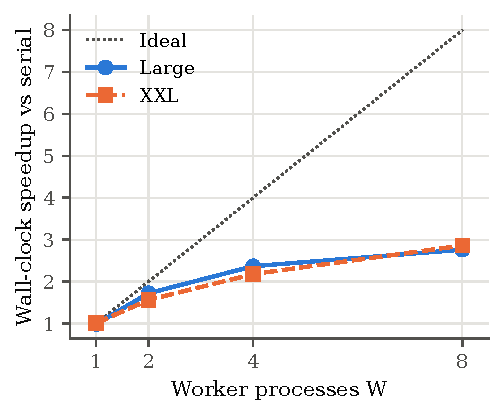
\includegraphics{../results/figures/fig_scaling.pdf}
\caption{Measured wall-clock speedup of \pcm{} [\mcc] against serial execution for a fixed number of epochs (Table~\ref{tab:scaling}).}
\label{fig:scaling}
\end{figure}

\begin{figure}[!htb]
\centering
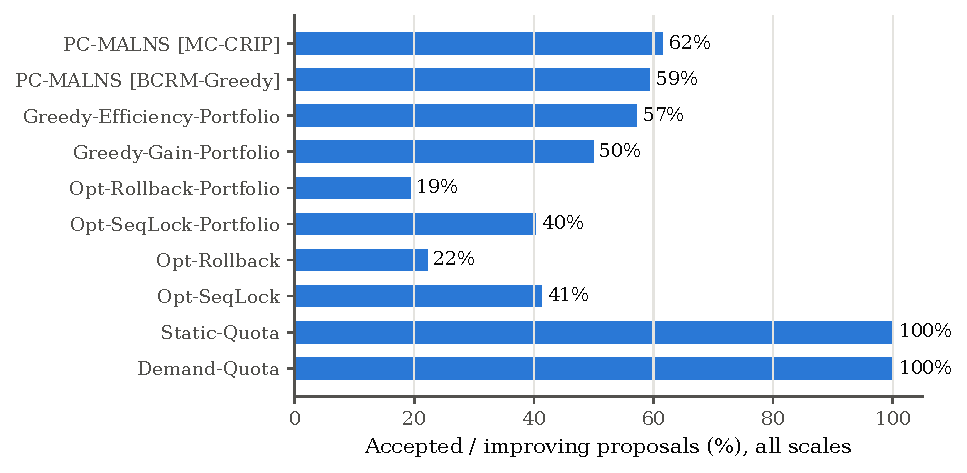
\includegraphics{../results/figures/fig_acceptance.pdf}
\caption{Committed improving moves per worker with an improving candidate (Table~\ref{tab:main}, all scales). The axis ends at $105\%$.}
\label{fig:acceptance}
\end{figure}

\subsection{Discussion}
\label{sec:discussion}
The study supports three practical conclusions. First, when concurrent LNS workers share capacities, letting each worker offer a few capacity-stratified alternatives and resolving them jointly is clearly better than optimistic commit or quotas; the size of the effect ($0.13$ to $0.17$ pp with the warm start, $1.3$ to $2.9$ pp from the cold start) grows with the share of conflict epochs. Second, how the barrier is resolved matters much less than offering the alternatives: an efficiency-sorted greedy pass is as good as or better than the exact program over whole runs, although it is worse in individual epochs. Third, against an exact solver the approach is competitive only under hard real-time limits and when the integer program is large relative to the budget, as with $20$ or $40$ candidates per request; with a few seconds more, HiGHS is better on compact instances. The main limitation is the improvement-only worker: it guarantees monotone descent but cannot release capacity at a local loss, which the MMKP instances expose. A coordinator that asks for such sacrifices, for example through capacity-buying levels priced by the barrier, is the most promising extension.

\section{Conclusion}
\label{sec:conclusion}
We studied the synchronization barrier of concurrent multi-agent LNS for block-angular multiple-choice allocation with shared capacities. In \pcm, workers send four capacity-stratified candidates and the barrier selects one per worker. Every epoch is feasible with monotone descent; the quotas cancel in the barrier constraint and serve only to diversify the portfolio; and the exact barrier dominates every other rule in each epoch, while greedy rules can be arbitrarily worse in a single epoch. In a controlled study with real multi-process execution, five runs per instance and exact tests, portfolio coordination beat optimistic rollback and sequential-lock commit on $56$ to $58$ of $60$ instances, also when these rules received the same portfolio, and beat static and demand-proportional quotas on all $60$. Counterfactual logging showed that the exact barrier gains about $20\%$ more per conflict epoch than greedy efficiency resolution, yet the greedy rule finished slightly better over whole runs in every family at the default tightness. Under budgets of $0.5$ to $6$ s on four processes, the method beat wall-clock-matched HiGHS on all $80$ instances with $20$ or $40$ candidates per request and on the larger six-candidate instances, whereas HiGHS was better with $5$ s or more on most compact instances and with equal CPU time on all of them. Prices and dynamic quotas gave no measurable gain, and the public MMKP instances revealed that improvement-only workers cannot trade capacity across agents. Future work should study barrier rules that look beyond the current epoch, workers that offer capacity-releasing sacrifices, and coarser tasks that reduce communication overhead.

\section*{CRediT authorship contribution statement}
\textbf{Naresh R:} Conceptualization, Methodology, Software, Validation, Formal analysis, Investigation, Data curation, Writing \textendash{} original draft, Writing \textendash{} review \& editing, Visualization.

\section*{Funding}
This research did not receive any specific grant from funding agencies in the public, commercial, or not-for-profit sectors.

\section*{Declaration of generative AI and AI-assisted technologies in the manuscript preparation process}
During the preparation of this work the author used Claude (Anthropic) and Gemini (Google) for language polishing, LaTeX formatting, and code debugging. After using these tools, the author reviewed and edited the content as needed and takes full responsibility for the content of the publication.

\section*{Declaration of competing interest}
The author declares that they have no known competing financial interests or personal relationships that could have appeared to influence the work reported in this paper.

\section*{Data and code availability}
The source code, the RPA-SH and RPA-SH-Sync instance generators, the MMKP conversion, all raw result files, the unit tests and the scripts that generate every table, figure and number of this paper are publicly available at \url{https://github.com/Naresh23032003/DG-MALNS}.

\appendix
\section{Implementation details}
\label{app:details}
All details are implemented in the public repository, in the modules \texttt{operators}, \texttt{worker}, \texttt{commit\_rules}, \texttt{bcrm\_solver}, \texttt{engine} and \texttt{agent\_pool} of the \texttt{src} directory.
\begin{itemize}[noitemsep]
    \item \textit{Destroy.} Worker $k$ removes $n_{\text{d}} = \max\{2, \operatorname{round}(f N_{\text{agent}})\}$ requests with $f \sim U(0.16, 0.30)$. First, $\min\{|C_k|, \max\{1, \lfloor 0.45\, n_{\text{d}} \rfloor\}\}$ consolidated requests ($C_k = \{i : p_i \ge 1\}$) with the largest score $2\sum_w A_{w,k,i,p_i} / \max\{1, c_{k,i,0} - c_{k,i,p_i}\} + U(0, 0.25)$ are removed; the remaining removals are the requests with the largest score $(c_{k,i,p_i} - \min_p c_{k,i,p}) + U(0.5, 18) + U(0, 22)$. Removed requests are set to $p = 0$.
    \item \textit{Regret-2 repair.} Each destroyed request gets the perturbed cost $\tilde{c}_{i,p} = c_{k,i,p} - c_{k,i,0} + \varepsilon_{i,p}$, $\varepsilon_{i,p} \sim N(0, \sigma^2)$, $\tilde{c}_{i,0} = 0$, with $\sigma = 2.0$ and $\sigma = 2.7$ for the two repairs of a best-of-two repair. In each step, for every unassigned request the candidates that respect the level's cap and $b_k$ are ranked; with best value $v_1$ and second-best value $v_2$, the request with the largest score $0.7(-v_1) + 0.3(v_2 - v_1)$ receives its best candidate. The borrower level adds the increase of the penalty in \eqref{eq:surrogate} to the value of a candidate. There is no limit on the number of consolidations per step.
    \item \textit{Chained steps.} Step $j \ge 2$ of a level destroys the level's current solution with the same destroy operator and repairs it against the cap minus the usage already consumed by the level; it is kept only if it lowers the agent's cost.
    \item \textit{Donor rebalance.} With hub weights $\nu = \mathbf{1}$ (or $\nu = \lambda^{(t)}$ with prices), up to two consolidated requests with the largest weighted burden per unit of saving, $\nu^\top D_{k,i,p_i} / (c_{k,i,0} - c_{k,i,p_i} + 1)$, move to their cheapest pattern $p'$ with $\nu^\top D_{k,i,p'} < \nu^\top D_{k,i,p_i}$; then one other request receives the upgrade with the largest saving whose added weighted usage does not exceed the released usage, subject to $b_k$.
    \item \textit{Barrier.} \mcc{} removes dominated levels and fixes agents with one remaining level; with at most $4{,}096$ combinations it enumerates, otherwise it calls HiGHS with relative gap $0$ and a $2$ s limit, with the fallback of Section~\ref{sec:barrier}. Ties in the greedy rules are broken by agent and level index.
    \item \textit{Counterfactual logging.} In each conflict epoch of a \pcm{} [\mcc] run, all rules are applied to the portfolios of the epoch; \texttt{Opt-Rollback} is evaluated by its exact expectation and \texttt{Opt-SeqLock} by the mean over $20$ random arrival orders, with a separate random stream. The logging time is subtracted from all clocks.
    \item \textit{Tolerances.} All feasibility checks use the absolute tolerance $10^{-6}$, and every committed selection and every final solution is verified.
\end{itemize}

\begin{thebibliography}{45}
\expandafter\ifx\csname natexlab\endcsname\relax\def\natexlab#1{#1}\fi
\providecommand{\url}[1]{\texttt{#1}}
\providecommand{\href}[2]{#2}
\providecommand{\path}[1]{#1}
\providecommand{\DOIprefix}{doi:}
\providecommand{\ArXivprefix}{arXiv:}
\providecommand{\URLprefix}{URL: }
\providecommand{\Pubmedprefix}{pmid:}
\providecommand{\doi}[1]{\href{http://dx.doi.org/#1}{\path{#1}}}
\providecommand{\bibinfo}[2]{#2}
\ifx\xfnm\relax \def\xfnm[#1]{\unskip,\space#1}\fi

\bibitem[{Alba(2005)}]{alba2005}
\bibinfo{author}{Alba, E.} (\bibinfo{year}{2005}).
\newblock \textit{\bibinfo{title}{Parallel Metaheuristics: A New Class of Algorithms}}.
\newblock \bibinfo{publisher}{John Wiley \& Sons}.

\bibitem[{Asokan et~al.(2014)Asokan, Furman, Goel, Li, \& Shao}]{asokan2014}
\bibinfo{author}{Asokan, B.~V.}, \bibinfo{author}{Furman, K.~C.}, \bibinfo{author}{Goel, V.}, \bibinfo{author}{Li, G.}, \& \bibinfo{author}{Shao, Y.} (\bibinfo{year}{2014}).
\newblock \bibinfo{title}{Parallel large-neighborhood search techniques for {LNG} inventory routing}.
\newblock \textit{\bibinfo{journal}{Optimization Online}}, \bibinfo{pages}{4319}.

\bibitem[{Bartodziej et~al.(2010)Bartodziej, Derigs, \& Vogel}]{bartodziej2010}
\bibinfo{author}{Bartodziej, P.}, \bibinfo{author}{Derigs, U.}, \& \bibinfo{author}{Vogel, U.} (\bibinfo{year}{2010}).
\newblock \bibinfo{title}{On the potentials of parallelizing large neighbourhood search for rich vehicle routing problems}.
\newblock In \textit{\bibinfo{booktitle}{Learning and Intelligent Optimization (LION 4)}}, Lecture Notes in Computer Science 6073 (pp. \bibinfo{pages}{216--219}). \bibinfo{publisher}{Springer}.

\bibitem[{Berthold(2013)}]{berthold2013}
\bibinfo{author}{Berthold, T.} (\bibinfo{year}{2013}).
\newblock \bibinfo{title}{Measuring the impact of primal heuristics}.
\newblock \textit{\bibinfo{journal}{Operations Research Letters}}, \bibinfo{volume}{41}(\bibinfo{number}{6}), \bibinfo{pages}{611--614}.

\bibitem[{Bertsekas(1982)}]{bertsekas1982}
\bibinfo{author}{Bertsekas, D.~P.} (\bibinfo{year}{1982}).
\newblock \textit{\bibinfo{title}{Constrained Optimization and Lagrange Multiplier Methods}}.
\newblock \bibinfo{publisher}{Academic Press}, \bibinfo{address}{New York}.

\bibitem[{Blum et~al.(2016)Blum, Pinacho, L{\'o}pez-Ib{\'a}{\~n}ez, \& Lozano}]{blum2016}
\bibinfo{author}{Blum, C.}, \bibinfo{author}{Pinacho, P.}, \bibinfo{author}{L{\'o}pez-Ib{\'a}{\~n}ez, M.}, \& \bibinfo{author}{Lozano, J.~A.} (\bibinfo{year}{2016}).
\newblock \bibinfo{title}{Construct, merge, solve \& adapt: A new general algorithm for combinatorial optimization}.
\newblock \textit{\bibinfo{journal}{Computers \& Operations Research}}, \bibinfo{volume}{68}, \bibinfo{pages}{75--88}.

\bibitem[{Boyd et~al.(2011)Boyd, Parikh, Chu, Peleato, \& Eckstein}]{boyd2011}
\bibinfo{author}{Boyd, S.}, \bibinfo{author}{Parikh, N.}, \bibinfo{author}{Chu, E.}, \bibinfo{author}{Peleato, B.}, \& \bibinfo{author}{Eckstein, J.} (\bibinfo{year}{2011}).
\newblock \bibinfo{title}{Distributed optimization and statistical learning via the alternating direction method of multipliers}.
\newblock \textit{\bibinfo{journal}{Foundations and Trends in Machine Learning}}, \bibinfo{volume}{3}(\bibinfo{number}{1}), \bibinfo{pages}{1--122}.

\bibitem[{Chan et~al.(2024)Chan, Chen, Lin, Zhang, Harabor, Koenig, Huang, \& Phan}]{chan2024}
\bibinfo{author}{Chan, S.-H.}, \bibinfo{author}{Chen, Z.}, \bibinfo{author}{Lin, D.-L.}, \bibinfo{author}{Zhang, Y.}, \bibinfo{author}{Harabor, D.}, \bibinfo{author}{Koenig, S.}, \bibinfo{author}{Huang, T.-W.}, \& \bibinfo{author}{Phan, T.} (\bibinfo{year}{2024}).
\newblock \bibinfo{title}{Anytime multi-agent path finding using operation parallelism in large neighborhood search}.
\newblock In \textit{\bibinfo{booktitle}{Proceedings of the 23rd International Conference on Autonomous Agents and Multiagent Systems (AAMAS 2024)}} (pp. \bibinfo{pages}{2183--2185}).

\bibitem[{Chen \& Hao(2014)}]{chen2014}
\bibinfo{author}{Chen, Y.}, \& \bibinfo{author}{Hao, J.-K.} (\bibinfo{year}{2014}).
\newblock \bibinfo{title}{A ``reduce and solve'' approach for the multiple-choice multidimensional knapsack problem}.
\newblock \textit{\bibinfo{journal}{European Journal of Operational Research}}, \bibinfo{volume}{239}(\bibinfo{number}{2}), \bibinfo{pages}{313--322}.

\bibitem[{Crainic(2019)}]{crainic2019}
\bibinfo{author}{Crainic, T.~G.} (\bibinfo{year}{2019}).
\newblock \bibinfo{title}{Parallel metaheuristics and cooperative search}.
\newblock In \textit{\bibinfo{booktitle}{Handbook of Metaheuristics}} (pp. \bibinfo{pages}{419--451}). \bibinfo{publisher}{Springer}.

\bibitem[{Falsone et~al.(2017)Falsone, Margellos, Garatti, \& Prandini}]{falsone2017}
\bibinfo{author}{Falsone, A.}, \bibinfo{author}{Margellos, K.}, \bibinfo{author}{Garatti, S.}, \& \bibinfo{author}{Prandini, M.} (\bibinfo{year}{2017}).
\newblock \bibinfo{title}{Dual decomposition for multi-agent distributed optimization with coupling constraints}.
\newblock \textit{\bibinfo{journal}{Automatica}}, \bibinfo{volume}{84}, \bibinfo{pages}{149--158}.

\bibitem[{Fioretto et~al.(2017)Fioretto, Dovier, Pontelli, Yeoh, \& Zivan}]{fioretto2017}
\bibinfo{author}{Fioretto, F.}, \bibinfo{author}{Dovier, A.}, \bibinfo{author}{Pontelli, E.}, \bibinfo{author}{Yeoh, W.}, \& \bibinfo{author}{Zivan, R.} (\bibinfo{year}{2017}).
\newblock \bibinfo{title}{Solving {DCOPs} with distributed large neighborhood search}.
\newblock \textit{\bibinfo{journal}{arXiv preprint arXiv:1702.06915}}.

\bibitem[{Fioretto et~al.(2018)Fioretto, Pontelli, \& Yeoh}]{fioretto2018}
\bibinfo{author}{Fioretto, F.}, \bibinfo{author}{Pontelli, E.}, \& \bibinfo{author}{Yeoh, W.} (\bibinfo{year}{2018}).
\newblock \bibinfo{title}{Distributed constraint optimization problems and applications: A survey}.
\newblock \textit{\bibinfo{journal}{Journal of Artificial Intelligence Research}}, \bibinfo{volume}{61}, \bibinfo{pages}{623--698}.

\bibitem[{Fisher(1981)}]{fisher1981}
\bibinfo{author}{Fisher, M.~L.} (\bibinfo{year}{1981}).
\newblock \bibinfo{title}{The {Lagrangian} relaxation method for solving integer programming problems}.
\newblock \textit{\bibinfo{journal}{Management Science}}, \bibinfo{volume}{27}(\bibinfo{number}{1}), \bibinfo{pages}{1--18}.

\bibitem[{Gao et~al.(2017)Gao, Lu, Yao, \& Li}]{gao2017}
\bibinfo{author}{Gao, C.}, \bibinfo{author}{Lu, G.}, \bibinfo{author}{Yao, X.}, \& \bibinfo{author}{Li, J.} (\bibinfo{year}{2017}).
\newblock \bibinfo{title}{An iterative pseudo-gap enumeration approach for the multidimensional multiple-choice knapsack problem}.
\newblock \textit{\bibinfo{journal}{European Journal of Operational Research}}, \bibinfo{volume}{260}(\bibinfo{number}{1}), \bibinfo{pages}{1--11}.

\bibitem[{Geoffrion(1970)}]{geoffrion1970}
\bibinfo{author}{Geoffrion, A.~M.} (\bibinfo{year}{1970}).
\newblock \bibinfo{title}{Primal resource-directive approaches for optimizing nonlinear decomposable systems}.
\newblock \textit{\bibinfo{journal}{Operations Research}}, \bibinfo{volume}{18}(\bibinfo{number}{3}), \bibinfo{pages}{375--403}.

\bibitem[{Gro{\"e}r et~al.(2011)Gro{\"e}r, Golden, \& Wasil}]{groer2011}
\bibinfo{author}{Gro{\"e}r, C.}, \bibinfo{author}{Golden, B.}, \& \bibinfo{author}{Wasil, E.} (\bibinfo{year}{2011}).
\newblock \bibinfo{title}{A parallel algorithm for the vehicle routing problem}.
\newblock \textit{\bibinfo{journal}{INFORMS Journal on Computing}}, \bibinfo{volume}{23}(\bibinfo{number}{2}), \bibinfo{pages}{315--330}.

\bibitem[{Guignard(2003)}]{guignard2003}
\bibinfo{author}{Guignard, M.} (\bibinfo{year}{2003}).
\newblock \bibinfo{title}{Lagrangean relaxation}.
\newblock \textit{\bibinfo{journal}{TOP}}, \bibinfo{volume}{11}(\bibinfo{number}{2}), \bibinfo{pages}{151--200}.

\bibitem[{Held et~al.(1974)Held, Wolfe, \& Crowder}]{held1974}
\bibinfo{author}{Held, M.}, \bibinfo{author}{Wolfe, P.}, \& \bibinfo{author}{Crowder, H.~P.} (\bibinfo{year}{1974}).
\newblock \bibinfo{title}{Validation of subgradient optimization}.
\newblock \textit{\bibinfo{journal}{Mathematical Programming}}, \bibinfo{volume}{6}(\bibinfo{number}{1}), \bibinfo{pages}{62--88}.

\bibitem[{Hemmelmayr et~al.(2012)Hemmelmayr, Cordeau, \& Crainic}]{hemmelmayr2012}
\bibinfo{author}{Hemmelmayr, V.~C.}, \bibinfo{author}{Cordeau, J.-F.}, \& \bibinfo{author}{Crainic, T.~G.} (\bibinfo{year}{2012}).
\newblock \bibinfo{title}{An adaptive large neighborhood search heuristic for two-echelon vehicle routing problems arising in city logistics}.
\newblock \textit{\bibinfo{journal}{Computers \& Operations Research}}, \bibinfo{volume}{39}(\bibinfo{number}{12}), \bibinfo{pages}{3215--3228}.

\bibitem[{Hendel(2022)}]{hendel2022}
\bibinfo{author}{Hendel, G.} (\bibinfo{year}{2022}).
\newblock \bibinfo{title}{Adaptive large neighborhood search for mixed integer programming}.
\newblock \textit{\bibinfo{journal}{Mathematical Programming Computation}}, \bibinfo{volume}{14}(\bibinfo{number}{2}), \bibinfo{pages}{185--221}.

\bibitem[{Hifi et~al.(2004)Hifi, Michrafy, \& Sbihi}]{hifi2004}
\bibinfo{author}{Hifi, M.}, \bibinfo{author}{Michrafy, M.}, \& \bibinfo{author}{Sbihi, A.} (\bibinfo{year}{2004}).
\newblock \bibinfo{title}{Heuristic algorithms for the multiple-choice multidimensional knapsack problem}.
\newblock \textit{\bibinfo{journal}{Journal of the Operational Research Society}}, \bibinfo{volume}{55}(\bibinfo{number}{12}), \bibinfo{pages}{1323--1332}.

\bibitem[{Hifi et~al.(2006)Hifi, Michrafy, \& Sbihi}]{hifi2006}
\bibinfo{author}{Hifi, M.}, \bibinfo{author}{Michrafy, M.}, \& \bibinfo{author}{Sbihi, A.} (\bibinfo{year}{2006}).
\newblock \bibinfo{title}{A reactive local search-based algorithm for the multiple-choice multi-dimensional knapsack problem}.
\newblock \textit{\bibinfo{journal}{Computational Optimization and Applications}}, \bibinfo{volume}{33}(\bibinfo{number}{2--3}), \bibinfo{pages}{271--285}.

\bibitem[{Hoang et~al.(2018)Hoang, Fioretto, Yeoh, Pontelli, \& Zivan}]{hoang2018}
\bibinfo{author}{Hoang, K.~D.}, \bibinfo{author}{Fioretto, F.}, \bibinfo{author}{Yeoh, W.}, \bibinfo{author}{Pontelli, E.}, \& \bibinfo{author}{Zivan, R.} (\bibinfo{year}{2018}).
\newblock \bibinfo{title}{A large neighboring search schema for multi-agent optimization}.
\newblock In \textit{\bibinfo{booktitle}{Principles and Practice of Constraint Programming (CP 2018)}} (pp. \bibinfo{pages}{688--706}). \bibinfo{publisher}{Springer}.

\bibitem[{Huangfu \& Hall(2018)}]{huangfu2018}
\bibinfo{author}{Huangfu, Q.}, \& \bibinfo{author}{Hall, J. A.~J.} (\bibinfo{year}{2018}).
\newblock \bibinfo{title}{Parallelizing the dual revised simplex method}.
\newblock \textit{\bibinfo{journal}{Mathematical Programming Computation}}, \bibinfo{volume}{10}(\bibinfo{number}{1}), \bibinfo{pages}{119--142}.

\bibitem[{Joncour et~al.(2010)Joncour, Michel, Sadykov, Sverdlov, \& Vanderbeck}]{joncour2010}
\bibinfo{author}{Joncour, C.}, \bibinfo{author}{Michel, S.}, \bibinfo{author}{Sadykov, R.}, \bibinfo{author}{Sverdlov, D.}, \& \bibinfo{author}{Vanderbeck, F.} (\bibinfo{year}{2010}).
\newblock \bibinfo{title}{Column generation based primal heuristics}.
\newblock \textit{\bibinfo{journal}{Electronic Notes in Discrete Mathematics}}, \bibinfo{volume}{36}, \bibinfo{pages}{695--702}.

\bibitem[{Khan et~al.(2002)Khan, Li, Manning, \& Akbar}]{khan2002}
\bibinfo{author}{Khan, S.}, \bibinfo{author}{Li, K.~F.}, \bibinfo{author}{Manning, E.~G.}, \& \bibinfo{author}{Akbar, M.~M.} (\bibinfo{year}{2002}).
\newblock \bibinfo{title}{Solving the knapsack problem for adaptive multimedia systems}.
\newblock \textit{\bibinfo{journal}{Studia Informatica Universalis}}, \bibinfo{volume}{2}(\bibinfo{number}{1}), \bibinfo{pages}{157--178}.

\bibitem[{Lahrichi et~al.(2015)Lahrichi, Crainic, Gendreau, Rei, Crisan, \& Vidal}]{lahrichi2015}
\bibinfo{author}{Lahrichi, N.}, \bibinfo{author}{Crainic, T.~G.}, \bibinfo{author}{Gendreau, M.}, \bibinfo{author}{Rei, W.}, \bibinfo{author}{Crisan, G.~C.}, \& \bibinfo{author}{Vidal, T.} (\bibinfo{year}{2015}).
\newblock \bibinfo{title}{An integrative cooperative search framework for multi-decision-attribute combinatorial optimization: Application to the {MDPVRP}}.
\newblock \textit{\bibinfo{journal}{European Journal of Operational Research}}, \bibinfo{volume}{246}(\bibinfo{number}{2}), \bibinfo{pages}{400--412}.

\bibitem[{Lamanna et~al.(2022)Lamanna, Mansini, \& Zanotti}]{lamanna2022}
\bibinfo{author}{Lamanna, L.}, \bibinfo{author}{Mansini, R.}, \& \bibinfo{author}{Zanotti, R.} (\bibinfo{year}{2022}).
\newblock \bibinfo{title}{A two-phase kernel search variant for the multidimensional multiple-choice knapsack problem}.
\newblock \textit{\bibinfo{journal}{European Journal of Operational Research}}, \bibinfo{volume}{297}(\bibinfo{number}{1}), \bibinfo{pages}{53--65}.

\bibitem[{Li et~al.(2021)Li, Chen, Harabor, Stuckey, \& Koenig}]{li2021}
\bibinfo{author}{Li, J.}, \bibinfo{author}{Chen, Z.}, \bibinfo{author}{Harabor, D.}, \bibinfo{author}{Stuckey, P.~J.}, \& \bibinfo{author}{Koenig, S.} (\bibinfo{year}{2021}).
\newblock \bibinfo{title}{Anytime multi-agent path finding via large neighborhood search}.
\newblock In \textit{\bibinfo{booktitle}{Proceedings of the 30th International Joint Conference on Artificial Intelligence (IJCAI 2021)}} (pp. \bibinfo{pages}{4127--4135}).

\bibitem[{Mansini \& Zanotti(2020)}]{mansini2020}
\bibinfo{author}{Mansini, R.}, \& \bibinfo{author}{Zanotti, R.} (\bibinfo{year}{2020}).
\newblock \bibinfo{title}{A core-based exact algorithm for the multidimensional multiple choice knapsack problem}.
\newblock \textit{\bibinfo{journal}{INFORMS Journal on Computing}}, \bibinfo{volume}{32}(\bibinfo{number}{4}), \bibinfo{pages}{1061--1079}.

\bibitem[{Masson et~al.(2013)Masson, Lehu{\'e}d{\'e}, \& P{\'e}ton}]{masson2013}
\bibinfo{author}{Masson, R.}, \bibinfo{author}{Lehu{\'e}d{\'e}, F.}, \& \bibinfo{author}{P{\'e}ton, O.} (\bibinfo{year}{2013}).
\newblock \bibinfo{title}{An adaptive large neighborhood search for the pickup and delivery problem with transfers}.
\newblock \textit{\bibinfo{journal}{Transportation Science}}, \bibinfo{volume}{47}(\bibinfo{number}{3}), \bibinfo{pages}{344--355}.

\bibitem[{Pisinger \& R{\o}pke(2007)}]{pisinger2007}
\bibinfo{author}{Pisinger, D.}, \& \bibinfo{author}{R{\o}pke, S.} (\bibinfo{year}{2007}).
\newblock \bibinfo{title}{A general heuristic for vehicle routing problems}.
\newblock \textit{\bibinfo{journal}{Computers \& Operations Research}}, \bibinfo{volume}{34}(\bibinfo{number}{8}), \bibinfo{pages}{2403--2435}.

\bibitem[{Polyak(1969)}]{polyak1969}
\bibinfo{author}{Polyak, B.~T.} (\bibinfo{year}{1969}).
\newblock \bibinfo{title}{Minimization of unsmooth functionals}.
\newblock \textit{\bibinfo{journal}{USSR Computational Mathematics and Mathematical Physics}}, \bibinfo{volume}{9}(\bibinfo{number}{3}), \bibinfo{pages}{14--29}.

\bibitem[{Potvin \& Rousseau(1993)}]{potvin1993}
\bibinfo{author}{Potvin, J.-Y.}, \& \bibinfo{author}{Rousseau, J.-M.} (\bibinfo{year}{1993}).
\newblock \bibinfo{title}{A parallel route building algorithm for the vehicle routing and scheduling problem with time windows}.
\newblock \textit{\bibinfo{journal}{European Journal of Operational Research}}, \bibinfo{volume}{66}(\bibinfo{number}{3}), \bibinfo{pages}{331--340}.

\bibitem[{R{\o}pke(2009)}]{ropke2009}
\bibinfo{author}{R{\o}pke, S.} (\bibinfo{year}{2009}).
\newblock \bibinfo{title}{{PALNS}: A software framework for parallel large neighborhood search}.
\newblock In \textit{\bibinfo{booktitle}{Proceedings of the 8th Metaheuristics International Conference (MIC 2009)}}, \bibinfo{note}{CD-ROM, pp. id-1--id-10}.

\bibitem[{R{\o}pke \& Pisinger(2006)}]{ropke2006}
\bibinfo{author}{R{\o}pke, S.}, \& \bibinfo{author}{Pisinger, D.} (\bibinfo{year}{2006}).
\newblock \bibinfo{title}{An adaptive large neighborhood search heuristic for the pickup and delivery problem with time windows}.
\newblock \textit{\bibinfo{journal}{Transportation Science}}, \bibinfo{volume}{40}(\bibinfo{number}{4}), \bibinfo{pages}{455--472}.

\bibitem[{Sadykov et~al.(2019)Sadykov, Vanderbeck, Pessoa, Tahiri, \& Uchoa}]{sadykov2019}
\bibinfo{author}{Sadykov, R.}, \bibinfo{author}{Vanderbeck, F.}, \bibinfo{author}{Pessoa, A.}, \bibinfo{author}{Tahiri, I.}, \& \bibinfo{author}{Uchoa, E.} (\bibinfo{year}{2019}).
\newblock \bibinfo{title}{Primal heuristics for branch and price: The assets of diving methods}.
\newblock \textit{\bibinfo{journal}{INFORMS Journal on Computing}}, \bibinfo{volume}{31}(\bibinfo{number}{2}), \bibinfo{pages}{251--267}.

\bibitem[{Santini et~al.(2018)Santini, R{\o}pke, \& Hvattum}]{santini2018}
\bibinfo{author}{Santini, A.}, \bibinfo{author}{R{\o}pke, S.}, \& \bibinfo{author}{Hvattum, L.~M.} (\bibinfo{year}{2018}).
\newblock \bibinfo{title}{A comparison of acceptance criteria for the adaptive large neighbourhood search metaheuristic}.
\newblock \textit{\bibinfo{journal}{Journal of Heuristics}}, \bibinfo{volume}{24}(\bibinfo{number}{5}), \bibinfo{pages}{783--815}.

\bibitem[{Schryen(2020)}]{schryen2020}
\bibinfo{author}{Schryen, G.} (\bibinfo{year}{2020}).
\newblock \bibinfo{title}{Parallel computational optimization in operations research: A new integrative framework, literature review and research directions}.
\newblock \textit{\bibinfo{journal}{European Journal of Operational Research}}, \bibinfo{volume}{287}(\bibinfo{number}{1}), \bibinfo{pages}{1--18}.

\bibitem[{Shaw(1998)}]{shaw1998}
\bibinfo{author}{Shaw, P.} (\bibinfo{year}{1998}).
\newblock \bibinfo{title}{Using constraint programming and local search methods to solve vehicle routing problems}.
\newblock In \textit{\bibinfo{booktitle}{Principles and Practice of Constraint Programming (CP 1998)}} (pp. \bibinfo{pages}{417--431}). \bibinfo{publisher}{Springer}.

\bibitem[{Vujanic et~al.(2016)Vujanic, Mohajerin~Esfahani, Goulart, Mari{\'e}thoz, \& Morari}]{vujanic2016}
\bibinfo{author}{Vujanic, R.}, \bibinfo{author}{Mohajerin~Esfahani, P.}, \bibinfo{author}{Goulart, P.~J.}, \bibinfo{author}{Mari{\'e}thoz, S.}, \& \bibinfo{author}{Morari, M.} (\bibinfo{year}{2016}).
\newblock \bibinfo{title}{A decomposition method for large scale {MILPs}, with performance guarantees and a power system application}.
\newblock \textit{\bibinfo{journal}{Automatica}}, \bibinfo{volume}{67}, \bibinfo{pages}{144--156}.

\end{thebibliography}

\end{document}
